\documentclass[grad,pdftex]{poli}
\usepackage[utf8]{inputenc}
\usepackage{amsmath,amssymb}
\usepackage{float}
\usepackage{multirow}
\usepackage{longtable}
\usepackage{tikz}
\usetikzlibrary{shapes,arrows,chains,positioning}
\usepackage{enumitem}
\usepackage{indentfirst}
\usepackage{array}
\usepackage{diagbox}
\usepackage[numbers,sort&compress]{natbib}
\usepackage{mciteplus}



\makelosymbols
\makeloabbreviations

\begin{document}
  \title{Biribá: Sistema web para a gestão do Programa de Aquisição de Alimentos}
  \foreigntitle{TCC Title}
  \author{Wilson}{Albuquerque Ramos}
  \advisor{Prof.}{Celso Alexandre}{Souza de Alvear}{D.Sc.}
\examiner{Prof.}{Nome Completo}{Ph.D.}
  \examiner{Prof.}{Nome Completo}{D.Sc.}
\department{DEL} \date{2}{2023}
  \keyword{Tecnologia social}
  \keyword{Software Livre}
  \keyword{Gestão comunitária}
  \keyword{Engenharia de software}
  \maketitle

  \frontmatter
\clearpage{}\chapter*{Agradecimentos}


O autor agradece a seus pais, Jocimar e Terezinha, por sempre lhe mostrarem o caminho dos estudos, e à sua esposa, Gabrielle, pelo apoio ao longo dessa trajetória.


O autor também agradece aos amigos que sempre estiveram ao seu lado, em especial àqueles que conheceu ao longo da graduação e que tornaram essa caminhada mais leve.


Por fim, este trabalho é dedicado ao povo brasileiro, que contribuiu de forma significativa para a formação e a permanência do autor nesta Universidade. Este projeto representa uma pequena forma de retribuir o investimento e a confiança nele depositados.

\clearpage{}
  \clearpage{}\begin{abstract}
    

O Programa de Aquisição de Alimentos é um projeto do governo federal que realiza compras diretas de alimentos dos agricultores familiares a preço de mercado sem a necessidade de licitações e distribui para pessoas em situação de insegurança alimentar, assim como a rede socioassistencial, equipamentos públicos e a rede pública de ensino. A fim de realizar a gestão do programa no assentamento PDS - Osvaldo de Oliveira, foi desenvolvido um sistema web que contemple todos os processos realizados pelos agricultores e o gestor responsável. Para o desenvolvimento do sistema foram usadas abordagens de engenharia de software, como levantamento de requisitos e metodologia ágil. O projeto segue o padrão arquitetural MVC, sendo o módulo responsável pelo processamento e armazenamento de dados e o módulo de interação com o usuário separados em containers. O deploy do projeto foi feito usando o GitLab actions para a geração da imagem e o envio para o servidor de homologação. Foram usados o Docker container para isolar os módulos e o Docker Compose para inicializar a aplicação. Todo o projeto é open source e está disponível no GitLab.


\end{abstract}
\clearpage{}
  \clearpage{}\begin{foreignabstract}

The Food Acquisition Program is a Brazilian federal government project that purchases food directly from family farmers at market prices, without the need for bidding processes, and distributes it to people experiencing food insecurity, as well as to the social assistance network, public facilities, and the public education system.

In order to manage the program in the PDS Osvaldo de Oliveira settlement, a web system was developed to cover all processes carried out by the farmers and the responsible manager. Software engineering approaches, such as requirements gathering and agile methodology, were used in the development of the system.

The project follows the MVC architectural pattern, with the module responsible for data processing and storage separated from the user interaction module in different containers. The project deployment was carried out using GitLab Actions to generate the image and send it to the staging server.

Docker containers were used to isolate the modules, and Docker Compose was used to start the application. The entire project is open source and available on GitLab.


\end{foreignabstract}

\clearpage{}
  \tableofcontents
  \listoffigures
  \listoftables
  \printlosymbols
  \printloabbreviations

  \mainmatter
    \clearpage{}\chapter{Introdução}

\section{Tema}

O Programa de Aquisição de Alimentos (PAA) é uma iniciativa do governo que tem como objetivo incentivar a agricultura familiar por meio de chamadas públicas e promover o acesso a uma alimentação saudável às famílias, sobretudo às que se encontram em situação de vulnerabilidade.

O gerenciamento de uma chamada pública do PAA requer organização e planejamento, visto que, ao longo do edital, são feitas entregas semanais de alimentos que devem ser registradas corretamente. Dito isso, este trabalho tem como objetivo descrever o sistema desenvolvido para gerenciar as entregas realizadas pelos agricultores a cada organização e equipamento de segurança alimentar que atendem à população em situação de insegurança alimentar e vulnerabilidade social.



\section{Delimitação}

O PAA possui seis modalidades no total. O projeto atuará na modalidade Doação Simultânea, que hoje é aplicada no assentamento dos agricultores do Projeto de Desenvolvimento Sustentável (PDS) Osvaldo de Oliveira, localizado no município de Macaé, na região Norte Fluminense.

\section{Justificativa}

Atualmente, a gestão da chamada pública em exercício no assentamento encontra-se centralizada em uma única pessoa, de modo que tarefas relacionadas às entregas semanais realizadas pelas famílias, à geração de comprovantes necessários para os atores do programa e ao monitoramento da chamada sobrecarregam seu trabalho e demandam tempo para serem realizadas.

\section{Objetivos}

Nesse contexto, o sistema tem como objetivo fornecer ao gestor um panorama geral do andamento do edital, padronizando a inserção de dados e sinalizando erros e inconsistências de forma visual, por meio de uma interface intuitiva. Além disso, automatiza a geração de comprovantes para os produtores, bem como da documentação necessária à validação das entregas.

\section{Metodologia}

O levantamento dos requisitos funcionais e não funcionais do sistema foi realizado por meio de reuniões com os coordenadores do PAA e a partir dos feedbacks fornecidos por eles ao longo do processo. Após o mapeamento das funcionalidades necessárias, tornou-se essencial definir as tecnologias a serem utilizadas no desenvolvimento, bem como o tipo de arquitetura a ser adotada.

Optou-se por uma arquitetura modular, garantindo a independência entre backend e frontend. No backend, foi escolhido o Java, uma linguagem consolidada no mercado, reconhecida por sua robustez, estabilidade e ampla comunidade, o que contribui para a manutenção e evolução do sistema. Para o frontend, adotou-se a biblioteca React, com o objetivo de proporcionar melhor performance e uma navegação mais fluida aos usuários. Como sistema gerenciador de banco de dados, utilizou-se o PostgreSQL, por se tratar de uma solução open source, estável, robusta e amplamente empregada em aplicações empresariais.

Todo o projeto foi versionado com o uso do Git e armazenado no GitLab. Cada módulo possui sua própria imagem Docker, armazenada no DockerHub. Para a integração contínua, geração das imagens e realização do deploy no ambiente de homologação, foi utilizado o GitLab CI/CD. Ressalta-se que todo o projeto é open source e pode ser clonado nos respectivos repositórios.


\section{Descrição}

No capítulo 2, são apresentados conceitos de Engenharia de Software relevantes para a construção do sistema. O capítulo aborda a importância do desenvolvimento de software de forma planejada e orientada à qualidade, discute processos de software, desenvolvimento ágil e apresenta a relação entre Software Livre, Código Aberto e continuidade tecnológica.

No capítulo 3, é discutida a arquitetura do sistema, com ênfase na organização modular da aplicação e na separação entre frontend, backend e banco de dados. Também são apresentadas as ferramentas de apoio ao desenvolvimento. No capítulo 4, são descritas as tecnologias utilizadas no desenvolvimento da plataforma. O capítulo reúne todas as ferramentas adotadas para o desenvolvimento.

No capítulo 5, é apresentada a implementação do sistema Biribá. São descritos todo o processo de desenvolvimento de software, desde o levantamento de requisitos até a implementação. No capítulo 6, são apresentados os resultados obtidos até o momento, destacando o estágio de homologação da aplicação e as funcionalidades implementadas.

Por fim, no capítulo 7, são apresentadas as conclusões do trabalho, retomando os objetivos alcançados juntamente com a contribuição do sistema para a redução de controles manuais e os trabalhos futuros necessários para o amadurecimento da ferramenta.
\clearpage{}
    \clearpage{}\chapter{Conceitos de Engenharia de Software}
\label{chap3}

\section{Engenharia de Software}

O software está presente no cotidiano do ser humano desde que os computadores e os sistemas embarcados se baratearam e ficaram mais acessíveis. Desenvolver nos dias de hoje com a chegada da inteligência artificial pode ser fácil e simples, desde que seja para uso pessoal. No entanto, quando se trata de softwares grandes, com demandas e comportamentos particulares, que resolvem problemas complexos, é necessário reconhecer a importância de um processo de desenvolvimento. A engenharia é tradicionalmente conhecida como a área que define processos e soluções para problemas complexos. Ou seja, o desenvolvimento de software profissional deve seguir padrões e conceitos da Engenharia de Software.

Essa necessidade de tratar o desenvolvimento de software como um processo organizado contribuiu para o surgimento do termo Engenharia de Software, apresentado na conferência da OTAN de 1968. O termo surgiu devido à demanda de que softwares fossem construídos com base em princípios práticos e teóricos, como todo produto de engenharia. De acordo com Sommerville (2018, p. 19), a Engenharia de Software pode ser definida como uma disciplina de engenharia que se preocupa com os aspectos da produção de software, desde sua concepção inicial até sua operação e manutenção. Com o desenvolvimento da área e sua consolidação como campo de conhecimento, a IEEE Computer Society, em parceria com a ACM, iniciou em 1998 o projeto SWEBOK, Guide to the Software Engineering Body of Knowledge, com o objetivo de organizar e formalizar os principais conhecimentos relacionados à Engenharia de Software. Esse movimento evidencia que a área passou a envolver diferentes dimensões do desenvolvimento, como requisitos, projeto, construção, testes, qualidade, manutenção, processos, métodos, ferramentas, gerência de configuração e gerência de engenharia de software, mostrando que a construção de sistemas exige mais do que apenas a implementação do código.

Mesmo com esse avanço na definição de processos, é consenso que não há uma bala de prata quando se trata da construção de um software, visto que cada problema tem uma particularidade e uma demanda, o que se reflete na construção do software. Softwares de caráter crítico, como, por exemplo, o sistema de piloto automático de uma aeronave, não devem ser construídos do mesmo modo que páginas web. Contudo, podem-se destacar propriedades que foram elencadas ao longo do tempo para o desenvolvimento de bons softwares, seja qual for o tipo. São elas: planejamento e objetivo claro; os sistemas devem ser resultado de um processo gerenciável e de fácil compreensão. O software deve se comportar do modo esperado e estar disponível sempre que necessário, além de ser seguro, prevenindo ataques externos. É necessário controlar e compreender especificações e requisitos do sistema. Por último, o software deve funcionar de modo eficaz e sempre deve reutilizar recursos que já tenham sido desenvolvidos para não reinventar a roda.


\section{Processos de software}

Os processos de software correspondem às formas pelas quais as atividades de desenvolvimento são organizadas e conduzidas ao longo de um projeto. Enquanto a Engenharia de Software estabelece uma perspectiva mais ampla sobre a produção de sistemas de qualidade, os processos dizem respeito à maneira concreta como o trabalho é estruturado, distribuído e acompanhado na prática, oferencendo referenciais para orientar a execução do projeto, favorecendo a coordenação entre os participantes e tornando o desenvolvimento mais compreensível além de controlável.

De modo geral, os processos de software envolvem atividades relacionadas à definição do que será construído,  à implementação da solução, à verificação de seu funcionamento e às modificações necessárias após as primeiras entregas. Essas atividades não se apresentam da mesma forma em todos os projetos, pois variam conforme o contexto, a natureza do sistema e a forma de organização da equipe. Por isso, a noção de processo não deve ser associada a uma sequência rígida e única de etapas, mas a um conjunto de práticas que orienta o desenvolvimento de acordo com determinadas escolhas metodológicas.

Entre os modelos de processo mais conhecidos, destaca-se o modelo em cascata, baseado na execução sequencial das fases de desenvolvimento, o que favorece maior formalização e planejamento prévio. Essa abordagem tende a ser mais adequada em situações nas quais o escopo está claramente definido e há baixa expectativa de mudança. Em contrapartida, sua estrutura linear dificulta ajustes ao longo do processo, especialmente em projetos marcados por incertezas. Como alternativa, consolidaram-se abordagens iterativas e ágeis, orientadas por ciclos mais curtos, entregas frequentes e acompanhamento contínuo do trabalho. Desse modo, a escolha do processo depende das características do projeto e do contexto em que ele se insere, não havendo um modelo único capaz de atender adequadamente a todas as situações.

\section{Desenvolvimento ágil de software}

O desenvolvimento ágil de software corresponde a uma forma de organização do trabalho voltada à adaptação contínua, à colaboração entre os participantes do projeto e à entrega frequente de resultados utilizáveis. Diferentemente de abordagens centradas em planejamento rígido e definição prévia de todas as etapas, a perspectiva ágil parte do entendimento de que o desenvolvimento ocorre em contextos dinâmicos, nos quais necessidades, prioridades e restrições podem se modificar ao longo do processo. Por essa razão, valoriza-se a capacidade de ajustar o percurso do projeto de maneira progressiva, sem perder de vista a coerência técnica e os objetivos da solução.

Nessa abordagem, a comunicação entre equipe, usuários e demais envolvidos assume papel central. O desenvolvimento deixa de ser compreendido como mera execução sequencial de atividades previamente fixadas e passa a ser conduzido por ciclos curtos de trabalho, nos quais a construção, a avaliação e o refinamento da solução ocorrem de forma recorrente. Essa dinâmica favorece o alinhamento entre o que está sendo produzido e as necessidades efetivas do contexto de uso, além de permitir correções de rumo ao longo do projeto.

Outro aspecto característico do desenvolvimento ágil é sua base iterativa e incremental. Em vez de concentrar a validação apenas ao final do processo, a solução é construída em partes menores, que podem ser implementadas, avaliadas e aperfeiçoadas sucessivamente. Esse modo de organização contribui para a identificação antecipada de problemas, para a incorporação mais rápida de feedback e para a redução de riscos associados a interpretações inadequadas dos requisitos. Ao mesmo tempo, amplia a possibilidade de entregas parciais com valor prático, tornando o processo mais sensível às transformações do ambiente e às demandas que emergem no decorrer do trabalho.

Entre as principais formas de operacionalização do desenvolvimento ágil, destacam-se o Scrum, o Kanban e o Extreme Programming (XP). O Scrum estrutura o trabalho em ciclos curtos, com momentos regulares de planejamento, acompanhamento e revisão, favorecendo a adaptação contínua das prioridades. O Kanban enfatiza a visualização do fluxo de atividades, o controle do trabalho em andamento e a melhoria contínua do processo. Já o XP concentra-se mais diretamente em práticas técnicas de desenvolvimento, como testes frequentes, refatoração contínua e colaboração intensa entre os membros da equipe. Embora apresentem ênfases distintas, essas abordagens compartilham princípios comuns do ágil, como desenvolvimento incremental, resposta rápida a mudanças, interação constante entre os envolvidos e busca contínua de alinhamento entre a solução produzida e as necessidades do contexto.

Entretanto, a adoção dessa abordagem não implica ausência de método ou informalidade excessiva. A flexibilidade característica do desenvolvimento ágil exige coordenação, definição de prioridades, comprometimento da equipe e mecanismos contínuos de acompanhamento. Sua efetividade depende, portanto, da capacidade de conciliar adaptação com disciplina técnica, preservando a qualidade da solução ao mesmo tempo em que se responde às mudanças do projeto.

\section{Software Livre e código aberto}

No campo do desenvolvimento de software, a discussão sobre Software Livre e Código Aberto insere-se de forma relevante entre os temas relacionados à produção, à circulação e à evolução de soluções computacionais. Para além dos aspectos estritamente técnicos, esses conceitos envolvem diferentes formas de acesso ao código-fonte, possibilidades de modificação do software e modos de compartilhamento da tecnologia. Nesse sentido, sua compreensão contribui para ampliar o debate sobre como sistemas são desenvolvidos, mantidos e apropriados por diferentes grupos ao longo do tempo.

O Software Livre corresponde da liberdade ao usuário para utilizar, estudar, modificar e redistribuir programas de computador. Assim, sua característica central não está associada à gratuidade, mas à garantia de autonomia sobre o uso e a transformação da tecnologia. Trata-se, portanto, de uma perspectiva que ultrapassa a dimensão estritamente operacional do software, incorporando também a possibilidade de compartilhamento do conhecimento, adaptação a diferentes contextos e fortalecimento da independência tecnológica. Essa característica torna o Software Livre  relevante em contextos nos quais a continuidade, a transparência e a possibilidade de adaptação da solução constituem aspectos importantes.O software deixa de ser entendido apenas como produto técnico fechado e passa a ser concebido como artefato passível de apropriação, modificação e evolução por diferentes atores, de acordo com necessidades específicas e mudanças de contexto.

O Open Source também se baseia na disponibilização do código-fonte e na possibilidade de modificação e redistribuição do software. Contudo, sua ênfase recai principalmente sobre as vantagens práticas desse modelo de desenvolvimento, como colaboração distribuída, aperfeiçoamento contínuo e maior flexibilidade na evolução das soluções. Já a noção de Software Livre atribui centralidade à liberdade dos usuários e ao valor social associado ao compartilhamento da tecnologia.

Desse modo, embora os dois conceitos sejam próximos e frequentemente apareçam associados, eles não são equivalentes. Ambos admitem abertura do código e contribuição coletiva, mas diferem quanto ao enfoque que orienta sua formulação. Enquanto o Open Source enfatiza os benefícios técnicos e organizacionais do desenvolvimento aberto, o Software Livre ressalta a autonomia, a circulação do conhecimento e a possibilidade de apropriação social da tecnologia. Essa distinção é relevante porque evidencia que a abertura do software pode ser compreendida tanto como estratégia de desenvolvimento quanto como compromisso com formas mais amplas de uso, adaptação e continuidade das soluções computacionais.

A adoção de Software Livre e de soluções Open Source também está diretamente relacionada ao tipo de licença que regula o uso, a modificação e a redistribuição do software. Essas licenças definem juridicamente as condições sob as quais o código pode ser utilizado por terceiros, influenciando o grau de liberdade, compartilhamento e reaproveitamento permitido. Entre as licenças mais conhecidas, destaca-se a licença MIT, caracterizada por maior permissividade, permitindo reutilização, modificação e redistribuição com poucas restrições. Em contraste, a licença GPL enfatiza a preservação das liberdades associadas ao software, exigindo que versões derivadas mantenham a mesma lógica de abertura do código. Dessa forma, as licenças não apenas regulamentam aspectos legais do software, mas também expressam diferentes entendimentos sobre colaboração, circulação do conhecimento e continuidade tecnológica.\clearpage{}
    \clearpage{}\chapter{Arquitetura do sistema}
\label{chap4}

\section{Visão Geral da Arquitetura}

A arquitetura de um sistema corresponde à forma como seus componentes são organizados e relacionados para atender aos requisitos funcionais e não funcionais da aplicação. No campo da Engenharia de Software, essa definição é importante porque a arquitetura não se restringe à estrutura técnica do sistema, mas influencia diretamente aspectos como manutenção, escalabilidade, evolução e integração com outras soluções. Nesse sentido, a definição arquitetural constitui uma etapa relevante do desenvolvimento, pois estabelece a base sobre a qual o sistema será construído e ampliado ao longo do tempo.

Entre as diferentes possibilidades de organização arquitetural, destaca-se a arquitetura modular, caracterizada pela divisão do sistema em partes com responsabilidades relativamente bem delimitadas. Essa abordagem favorece a separação de interesses, reduz o acoplamento entre componentes e facilita a compreensão, a manutenção e a evolução da aplicação. Além disso, a modularidade contribui para que novas funcionalidades possam ser incorporadas sem comprometer de forma significativa o funcionamento das partes já existentes, o que a torna especialmente adequada para sistemas que demandam crescimento progressivo e adaptação a diferentes contextos de uso.

No desenvolvimento de sistemas web, uma forma recorrente de materializar essa organização modular é a divisão entre frontend e backend. A camada de frontend é responsável pela interação com o usuário, concentrando os elementos visuais, os mecanismos de navegação e a apresentação das informações. Já a camada de backend concentra a lógica de negócio, o processamento das regras do sistema, o controle de acesso aos dados e a comunicação com o banco de dados. Essa separação contribui para distribuir responsabilidades de maneira mais clara, permitindo que interface e processamento interno evoluam com maior independência, ainda que permaneçam articulados no funcionamento da aplicação.

De modo complementar, a comunicação entre essas camadas costuma ocorrer por meio de interfaces de programação de aplicações, que permitem a troca estruturada de dados e favorecem a integração entre diferentes componentes e serviços. Em arquiteturas desse tipo, o banco de dados atua como mecanismo de persistência das informações, enquanto ferramentas de versionamento, conteinerização e automação de processos apoiam o desenvolvimento, a manutenção e a distribuição do sistema. Assim, a arquitetura modular em camadas constitui uma solução adequada para aplicações que exigem clareza estrutural, possibilidade de expansão e integração com outros sistemas. A organização geral dessa arquitetura será apresentada na figura a seguir.

\begin{figure}[H]
    \centering
    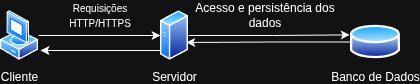
\includegraphics[width=0.5\linewidth]{Imagens/chap04/diagrama_cliente_servidor.png}
    \caption{Representação da arquitetura modular do sistema, cliente , servidor e banco de dados}
    \label{fig:arquitetura_cliente_servidor}
\end{figure}

\section{Camadas da Arquitetura do Sistema}

\subsection{Backend}

O backend corresponde à camada responsável pelo processamento das regras de negócio, pela validação dos dados recebidos, pelo controle de acesso e pela comunicação com os mecanismos de armazenamento e processamento de informações. Essa camada concentra a lógica central do sistema, garantindo que as operações sejam executadas de maneira consistente, segura e de acordo com os requisitos funcionais e não funcionais estabelecidos. Entre suas principais responsabilidades, destacam-se o tratamento e a persistência dos dados, a aplicação de restrições e validações, o gerenciamento de autenticação e autorização, o controle das transações, o tratamento de exceções e a disponibilização de serviços para outras camadas da arquitetura. Além disso, o backend contribui para atributos como integridade, confiabilidade, escalabilidade, segurança e manutenibilidade, constituindo um elemento fundamental para o funcionamento adequado de sistemas computacionais.


\subsection{Banco de Dados}

O banco de dados é o componente responsável pelo armazenamento persistente, pela organização e pela recuperação das informações utilizadas por um sistema. Trata-se de um elemento fundamental em aplicações computacionais, pois fornece a base necessária para o registro, a manutenção e o acesso estruturado aos dados. Além de armazenar informações de forma duradoura, o banco de dados também contribui para a integridade, a consistência, a segurança e a disponibilidade dos dados, permitindo que eles sejam consultados, atualizados e relacionados de maneira eficiente. Dessa forma, esse componente sustenta o funcionamento das demais camadas do sistema, servindo de apoio para o processamento realizado pela lógica da aplicação e para a disponibilização das informações aos usuários.


\subsection{Frontend}

O frontend corresponde à camada de apresentação do sistema, ou seja, à interface por meio da qual os usuários interagem com a aplicação. É nessa camada que se encontram os elementos visuais e interativos que possibilitam o uso do sistema, como telas, formulários, menus, listagens, botões e mecanismos de navegação. Sua principal função é apresentar informações e funcionalidades de forma compreensível, organizada e acessível, permitindo que a interação do usuário com o sistema ocorra de maneira eficiente e adequada ao seu contexto de uso. Além disso, o frontend também contribui para a usabilidade, a clareza na comunicação das informações, a responsividade da interface e a mediação entre as ações do usuário e os serviços disponibilizados pelas demais camadas da arquitetura.



\section{Ferramentas de Apoio ao Desenvolvimento}

\subsection{Controle de Versão}

O controle de versão é uma prática fundamental no desenvolvimento de software, pois permite registrar, organizar e acompanhar as alterações realizadas no código-fonte ao longo do tempo. Por meio desse processo, torna-se possível recuperar versões anteriores, comparar modificações, identificar a autoria das mudanças e manter um histórico estruturado da evolução do sistema. Além disso, o controle de versão desempenha papel essencial no trabalho colaborativo, uma vez que possibilita que diferentes desenvolvedores atuem simultaneamente sobre o mesmo projeto de forma coordenada, reduzindo conflitos e favorecendo a integração contínua das contribuições. Dessa maneira, essa prática contribui para a rastreabilidade, a segurança, a manutenção e a evolução consistente do software.


\subsection{Integração e Entrega Contínua (CI/CD)}

A integração contínua e a entrega contínua, frequentemente designadas pela sigla CI/CD, constituem práticas voltadas à automação e à padronização de etapas do ciclo de desenvolvimento de software. De modo geral, essas práticas buscam assegurar que alterações no código sejam integradas, verificadas e disponibilizadas de forma frequente e controlada, reduzindo a dependência de procedimentos manuais e tornando o processo de desenvolvimento mais confiável. A integração contínua está associada à incorporação recorrente de mudanças em um repositório compartilhado, normalmente acompanhada da execução automática de testes e validações. Já a entrega contínua se relaciona à preparação do software para que novas versões possam ser disponibilizadas de maneira rápida e consistente. Em conjunto, essas práticas contribuem para a detecção antecipada de falhas, para a melhoria da qualidade do software, para a redução de riscos nas liberações e para o aumento da previsibilidade e da eficiência no processo de desenvolvimento.

\subsection{Conteinerização e Distribuição }

A conteinerização consiste em empacotar aplicações, bibliotecas, arquivos de configuração e demais dependências em unidades padronizadas de execução, denominadas contêineres. Essa abordagem permite que o software seja executado de forma mais consistente em diferentes ambientes computacionais, reduzindo incompatibilidades entre desenvolvimento, teste e produção. Ao isolar a aplicação e os elementos necessários ao seu funcionamento, a conteinerização favorece a portabilidade, a padronização e a reprodutibilidade, além de contribuir para a escalabilidade, a eficiência na implantação e a simplificação do gerenciamento dos ambientes. Dessa forma, constitui uma prática amplamente adotada para tornar a distribuição e a execução de sistemas mais previsíveis, controladas e independentes das particularidades da infraestrutura subjacente.\clearpage{}
    \clearpage{}\chapter{Tecnologias}
\label{chap2}

\section{Tecnologias de desenvolvimento backend}

\subsection{Java 17}

O Java 17 é uma linguagem de programação orientada a objetos amplamente utilizada no desenvolvimento de sistemas corporativos e aplicações de grande porte. Por se tratar de uma versão de suporte de longo prazo (\textit{Long-Term Support} -- LTS), oferece maior estabilidade, segurança e compatibilidade para projetos que demandam manutenção contínua. Sua adoção contribui para a construção de aplicações robustas, portáveis e com amplo suporte do ecossistema de desenvolvimento.

\subsection{Spring Boot 3}

O Spring Boot 3 é um framework voltado à simplificação do desenvolvimento de aplicações baseadas na plataforma Spring. Sua principal proposta é reduzir a complexidade de configuração inicial, permitindo a criação de sistemas com maior agilidade e padronização. Além disso, fornece mecanismos que facilitam a organização modular da aplicação, a integração entre componentes e a configuração automatizada de diversos recursos.

\subsection{Spring Web}

O Spring Web é o módulo responsável pelo desenvolvimento da camada de comunicação da aplicação, especialmente no que se refere à construção de APIs e ao tratamento de requisições e respostas. Ele possibilita a definição de controladores, rotas e mecanismos de entrada e saída de dados, servindo como base para a interação entre clientes e serviços do sistema.

\subsection{Spring Data JPA / Hibernate}

O Spring Data JPA é uma tecnologia que simplifica o acesso e a manipulação de dados em aplicações Java, oferecendo uma abstração para operações de persistência. Em conjunto com o Hibernate, que atua como implementação do mapeamento objeto-relacional, permite relacionar entidades do sistema com tabelas do banco de dados. Essa combinação reduz a necessidade de escrita manual de consultas básicas, favorecendo produtividade, organização e manutenção do código.

\subsection{Spring Security}

O Spring Security é um framework voltado à segurança de aplicações, oferecendo mecanismos para autenticação, autorização e proteção de recursos. Seu uso permite controlar o acesso às funcionalidades do sistema com base em perfis, permissões e regras previamente definidas. Dessa forma, contribui para reforçar a proteção da aplicação contra acessos indevidos e para estruturar de maneira consistente as políticas de segurança adotadas.

\subsection{JWT}

O JWT (\textit{JSON Web Token}) é um padrão utilizado para representação segura de informações entre partes, sendo amplamente empregado em processos de autenticação e autorização. No contexto de sistemas distribuídos, ele permite que informações sobre a identidade do usuário e suas permissões sejam transmitidas de forma assinada, favorecendo a verificação de acesso sem a necessidade de armazenamento contínuo de sessão no servidor.

\subsection{PostgreSQL}

O PostgreSQL é um sistema gerenciador de banco de dados relacional de código aberto, reconhecido por sua confiabilidade, desempenho e conformidade com padrões SQL. Ele oferece recursos avançados para armazenamento, consulta, integridade e segurança dos dados, sendo amplamente utilizado em aplicações que exigem consistência e escalabilidade na persistência das informações.

\subsection{OpenAPI / Swagger}

O OpenAPI é uma especificação voltada à descrição padronizada de interfaces de programação de aplicações (\textit{Application Programming Interfaces} -- APIs). O Swagger, por sua vez, corresponde a um conjunto de ferramentas que possibilita visualizar, documentar e testar APIs com base nessa especificação. O uso dessas tecnologias favorece a clareza na definição dos contratos da aplicação, facilita a comunicação entre equipes e contribui para a validação e o consumo dos serviços disponibilizados.

\subsection{Maven}

O Maven é uma ferramenta de automação e gerenciamento de projetos utilizada principalmente em aplicações Java. Sua função envolve o controle de dependências, a padronização da estrutura do projeto e a automação de tarefas como compilação, testes e empacotamento. Dessa maneira, contribui para a organização do processo de desenvolvimento e para a reprodutibilidade da construção do software.

\subsection{JUnit / Mockito}

O JUnit é um framework amplamente utilizado para a elaboração e execução de testes automatizados em aplicações Java, especialmente testes unitários. O Mockito, por sua vez, complementa esse processo ao permitir a simulação de comportamentos de objetos e dependências externas. Em conjunto, essas ferramentas contribuem para a verificação do funcionamento do código, para o isolamento de componentes durante os testes e para o aumento da confiabilidade da aplicação.

\subsection{pgAdmin}

O pgAdmin é uma ferramenta gráfica de administração e gerenciamento do PostgreSQL. Sua utilização facilita atividades como visualização de tabelas, execução de consultas, monitoramento do banco e administração de estruturas de dados. Dessa forma, serve como apoio ao desenvolvimento e à manutenção do banco de dados, tornando mais acessíveis operações que poderiam ser realizadas apenas por linha de comando.

\section{Tecnologias de desenvolvimento frontend}

\subsection{React 19}

O React 19 é uma biblioteca JavaScript voltada à construção de interfaces de usuário baseadas em componentes reutilizáveis. Sua abordagem permite dividir a interface em partes independentes, facilitando a organização do código, a manutenção e a evolução da aplicação. Além disso, o React favorece a criação de interfaces dinâmicas e interativas, adequadas ao desenvolvimento de sistemas modernos.

\subsection{TypeScript}

O TypeScript é uma linguagem que estende o JavaScript por meio da adição de tipagem estática e outros recursos voltados à maior segurança no desenvolvimento. Sua utilização contribui para a detecção antecipada de erros, para a melhor documentação do código e para a maior previsibilidade no comportamento da aplicação. Dessa forma, favorece a manutenção e a escalabilidade de projetos de maior porte.

\subsection{Vite}

O Vite é uma ferramenta de construção e execução de aplicações frontend que se destaca pela rapidez no ambiente de desenvolvimento e pela simplicidade de configuração. Ele oferece suporte eficiente ao empacotamento do projeto, à atualização instantânea durante a codificação e à preparação da aplicação para produção. Seu uso contribui para tornar o processo de desenvolvimento mais ágil e produtivo.

\subsection{Material UI (MUI)}

O Material UI (MUI) é uma biblioteca de componentes visuais para aplicações React, baseada nos princípios do \textit{Material Design}. Ela oferece um conjunto de elementos de interface prontos, como botões, tabelas, campos de formulário, menus e diálogos, permitindo a construção de interfaces consistentes, responsivas e visualmente padronizadas. Seu uso contribui para acelerar o desenvolvimento e melhorar a usabilidade da aplicação.

\subsection{Emotion}

O Emotion é uma biblioteca voltada à estilização de interfaces em aplicações JavaScript e React. Ela permite definir estilos diretamente nos componentes, com flexibilidade para composição, reutilização e manutenção do design da aplicação. Essa abordagem favorece a organização dos estilos e a integração entre lógica e apresentação no desenvolvimento da interface.

\subsection{Redux Toolkit}

O Redux Toolkit é uma ferramenta destinada ao gerenciamento de estado global em aplicações frontend. Sua principal finalidade é simplificar o uso da arquitetura Redux, reduzindo a complexidade de configuração e de manipulação do estado compartilhado entre diferentes partes da aplicação. Dessa forma, contribui para a centralização das informações, para a previsibilidade do fluxo de dados e para a melhor organização do código.

\subsection{React Redux}

O React Redux é a biblioteca responsável por integrar o Redux às aplicações desenvolvidas com React. Ela fornece mecanismos para conectar componentes ao estado global da aplicação e para despachar ações que atualizam os dados compartilhados. Seu uso permite que a interface reaja de forma consistente às mudanças de estado, favorecendo a sincronização entre diferentes componentes.

\subsection{React Router DOM}

O React Router DOM é uma biblioteca utilizada para gerenciar a navegação entre diferentes páginas ou visualizações em aplicações React. Ela possibilita definir rotas, associar componentes a caminhos específicos e controlar a transição entre telas sem a necessidade de recarregamento completo da página. Dessa forma, contribui para a organização da navegação e para uma experiência de uso mais fluida.

\subsection{Axios}

O Axios é uma biblioteca utilizada para realizar requisições HTTP em aplicações JavaScript. No contexto do frontend, sua principal função é possibilitar a comunicação com serviços externos, como APIs responsáveis pelo fornecimento e recebimento de dados. Seu uso facilita o envio de requisições, o tratamento de respostas e o gerenciamento de erros na comunicação entre a interface e o backend.

\subsection{ESLint}

O ESLint é uma ferramenta de análise estática de código voltada à identificação de problemas de sintaxe, inconsistências e más práticas em projetos JavaScript e TypeScript. Sua utilização contribui para a padronização do código-fonte, para a melhoria da legibilidade e para a prevenção de erros durante o desenvolvimento. Assim, auxilia na manutenção da qualidade e da consistência do projeto.

\section{Tecnologias de Controle de Versão}


\subsection{Git}

O Git é um sistema de controle de versão distribuído amplamente utilizado no desenvolvimento de software para registrar, organizar e acompanhar as alterações realizadas no código-fonte ao longo do tempo. Por meio dele, torna-se possível manter um histórico detalhado das modificações, recuperar versões anteriores, criar ramificações independentes para desenvolvimento de funcionalidades e integrar mudanças de diferentes colaboradores de forma controlada. Sua utilização contribui para a rastreabilidade das alterações, para a segurança no processo de desenvolvimento e para a manutenção evolutiva do software.

\subsection{GitLab}

O GitLab é uma plataforma de hospedagem e gerenciamento de repositórios baseada no Git, que oferece recursos voltados ao desenvolvimento colaborativo e à automação de processos. Além de permitir o armazenamento centralizado do código-fonte, a ferramenta disponibiliza mecanismos para controle de acesso, revisão de código, gerenciamento de \textit{issues}, acompanhamento de atividades e integração com fluxos de integração contínua e entrega contínua. Dessa forma, o GitLab amplia as possibilidades de organização do projeto, de colaboração entre os membros da equipe e de controle do ciclo de desenvolvimento de software.

\section{Tecnologias de Conteinerização e Distribuição}

\subsection{Docker}

O Docker é uma plataforma voltada à conteinerização de aplicações, permitindo empacotar o software e suas dependências em unidades isoladas de execução, denominadas contêineres. No contexto de integração contínua e entrega contínua, seu uso contribui para a padronização dos ambientes de desenvolvimento, teste e implantação, reduzindo inconsistências entre diferentes etapas do ciclo de vida do software. Além disso, o Docker favorece a reprodutibilidade, a portabilidade e a escalabilidade da aplicação, tornando o processo de construção, validação e disponibilização de novas versões mais previsível e controlado.

\subsection{GitLab CI/CD}
O GitLab CI/CD corresponde ao conjunto de mecanismos de automação disponibilizados pela plataforma GitLab para apoiar práticas de integração contínua e entrega contínua. Por meio dessa abordagem, é possível definir fluxos automatizados para executar etapas como compilação, testes, validações e processos de implantação sempre que alterações são realizadas no repositório. Sua utilização contribui para reduzir atividades manuais, aumentar a confiabilidade do processo de desenvolvimento e permitir que a equipe acompanhe de forma mais sistemática a qualidade e a evolução do software. Dessa forma, o GitLab Actions fortalece a automação do ciclo de desenvolvimento e favorece a disponibilização mais rápida e consistente de novas versões da aplicação.\clearpage{}    
    \clearpage{}\chapter{Implementação}
\label{chap5}

O desenvolvimento do projeto teve início no segundo semestre de 2024, no âmbito da disciplina Software Livre e Metodologias Participativas. Após o término da disciplina, o projeto passou a integrar as atividades do projeto de extensão Tecnologia da Informação, Democracia e Movimentos Sociais (TICDeMoS), vinculado ao SOLTEC/UFRJ. Desde o início, a proposta contou com o acompanhamento da antiga gestora do PAA no PDS Osvaldo de Oliveira, que contribuiu com sua experiência para a modelagem do sistema e para a definição dos principais casos de uso.

Ao longo do desenvolvimento, a proposta passou por mudanças em sua organização técnica e funcional. Inicialmente, o sistema estava voltado para um único assentamento e para a criação de uma base mínima que permitisse cadastrar usuários, famílias, produtos, ciclos, destinos e editais. Em 2025, a proposta foi apresentada à equipe da Companhia Nacional de Abastecimento do Rio de Janeiro (CONAB-RJ). A reunião evidenciou a necessidade de contemplar, além do cadastro das informações essenciais do edital, o cadastro de coletivos, um painel que apresentasse com clareza o andamento do projeto e a geração de relatórios que apoiassem a comprovação das entregas, a visualização dos valores a receber pelas famílias agricultoras e a consolidação dos dados de entrega pelo coordenador.


\section{Requisitos do Sistema}

O levantamento dos requisitos do sistema foi realizado a partir de duas frentes diferentes, a primeira através de diálogo com a gestora do PAA no assentamento para entender seu dia-a-dia e como funcionava o diálogo com os agricultores e a segunda da análise baseado em planilhas no excel que mostrava o funcionamento da gestão do programa no Assentamento PDS Osvaldo de Oliveira. Inicialmente, o foco era entender como as informações das chamadas públicas eram organizadas, quais atividades eram realizadas durante a execução dos editais e quais dificuldades estavam presentes no processo de acompanhamento. Observou-se que o gerenciamento do edital envolve diferentes informações, como quais famílias agricultoras estão participando, quais produtos foram selecionados, quantas entregas foram realizadas, quais destinos receberão os alimentos e quais são os valores a receber por agricultor, além das informações para o gerenciamento do edital, era necessário gerar documentos que comprovassem as entregas.

\subsection{Casos de uso do sistema}

Os casos de uso do sistema foram definidos a partir das principais ações realizadas durante a gestão de uma chamada pública do PAA e para que ficasse coerente com o levantamento de requisitos. Como objetivo do sistema é organizar informações sobre editais, famílias, produtos, ciclos, destinos e entregas, foi necessário identificar quais pessoas interagem com a plataforma e quais atividades cada uma delas precisa realizar, que se resume em três atores principais, o administrador, o coordenador e o agricultor.

O administrador é o usuário que tem máximo acesso ao sistema, podendo criar coletivos, produtos, editais, aprovar usuários e modificar informações livremente no sistema. O segundo ator, o coordenador, é responsável por acompanhar a execução do edital, aprovar usuários do mesmo coletivo, cadastrar famílias, organizar produtos, criar editais, criar ciclos de entrega, registrar informações e acompanhar o andamento da chamada pública. Por fim, o agricultor acompanha as informações referentes à sua participação, como produtos previstos, entregas realizadas e valores a receber.

O primeiro caso de uso é o cadastro de usuários. Por meio dessa funcionalidade, uma pessoa interessada em acessar o sistema informa seus dados e solicita a criação de uma conta. Após esse cadastro, o usuário não recebe acesso imediato às funcionalidades internas, pois sua entrada depende da aprovação do coordenador/administrador.

O segundo caso de uso é a aprovação de usuários. Essa funcionalidade permite que o coordenador visualize os usuários cadastrados do mesmo coletivo e aprove ou rejeite o acesso à plataforma. Essa etapa é crucial para manter a segurança do sistema e garantir que apenas pessoas vinculadas ao processo de participação no PAA possam acessar as informações.

Outro caso de uso central é o cadastro e gerenciamento de famílias. Essa funcionalidade permite registrar as famílias agricultoras no sistema, editar suas informações e associar usuários a uma determinada família. Esse vínculo é necessário para que o sistema consiga relacionar as entregas, os produtos e os valores a cada unidade produtiva.

O sistema também possui o caso de uso relacionado à criação e gerenciamento de editais. O edital representa a chamada pública do PAA e reúne as principais informações do processo. A partir dele, são organizados os produtos, os destinos, os ciclos e as entregas.

O cadastro de produtos no sistema também é um dos principais casos de uso. Nele, o administrador registra os produtos que fazem parte do sistema e que são utilizados para a vinculação a um edital.

O cadastro de destinos também compõe os principais casos de uso. Essa funcionalidade permite registrar as organizações e equipamentos de segurança alimentar que receberão os alimentos.

A criação de ciclos de entrega é outro caso de uso fundamental. Como as entregas do PAA ocorrem de forma periódica, geralmente semanal, o sistema precisa organizar o edital em ciclos. Cada ciclo representa uma etapa de entrega e permite registrar os produtos movimentados em determinado período.

O registro das entregas realizadas representa uma das funcionalidades mais importantes do sistema. Por meio desse caso de uso, o coordenador informa quais famílias entregaram produtos, quais produtos foram entregues, em quais quantidades e para quais destinos. A partir desses dados, o sistema pode consolidar informações sobre o andamento do edital e calcular os valores correspondentes.

Também foi definido o caso de uso de acompanhamento do edital por meio de um dashboard. Esse dashboard tem como objetivo apresentar de forma visual e organizada o andamento da chamada pública, indicando informações como produtos entregues, valores acumulados, famílias participantes e ciclos já realizados.


Os casos de uso e as associações entre os atores e as funcionalidades são representados pelos diagramas UML do Apêndice~\ref{apendice-casos-uso}. Para facilitar a leitura, os casos foram organizados em quatro áreas funcionais: acesso ao sistema (Figura~\ref{fig:uc-acesso}), configuração do edital (Figura~\ref{fig:uc-configuracao}), execução e acompanhamento (Figura~\ref{fig:uc-execucao}) e administração da plataforma (Figura~\ref{fig:uc-administracao}).

\section{Modelagem do domínio e estrutura dos dados}

A modelagem do domínio foi construída a fim de atender às demandas necessárias para o acompanhamento do edital. O edital foi definido como uma das entidades centrais do sistema, pois representa a chamada pública que será gerenciada. Diretamente associado ao edital está o plano original, entidade que contém os produtos previstos, os destinos das entregas e as famílias participantes.

O plano original é uma entidade que formaliza o início do edital, com informações essenciais como quais famílias irão participar, quais produtos e quais serão os destinos dos alimentos.

As famílias representam um grupo de usuários agricultores que participam do PAA. Entre os usuários pertencentes a uma família, a entidade representante sinaliza qual deles será responsável pelos registros nos relatórios gerados. Essa relação é importante porque as entregas e os valores a receber precisam ser vinculados corretamente ao responsável da família pela produção.

A entidade produto representa cada alimento que faz parte da chamada pública. No sistema, os produtos podem ser cadastrados independentemente como valores globais no sistema e podem ser associados ao edital com informações como valor unitário e quantidade prevista. Essa associação permite diferenciar os produtos dos diversos editais, controlar o que foi planejado e comparar posteriormente com o que foi efetivamente entregue.

Os destinos representam as organizações, instituições ou equipamentos de segurança alimentar que recebem os alimentos. O registro dos destinos permite acompanhar para onde os produtos estão sendo encaminhados e quanto cada destino irá receber.

Os ciclos de entrega foram modelados para representar a periodicidade das entregas realizadas durante a execução do edital. Como as chamadas públicas podem envolver entregas semanais ao longo de vários meses, a divisão em ciclos permite organizar melhor o acompanhamento do processo. Cada ciclo corresponde a um período específico e pode reunir diferentes entregas, produtos, famílias e destinos.

A entrega representa o registro efetivo dos produtos fornecidos em determinado ciclo. Por meio dela, o sistema armazena quais produtos foram entregues, em quais quantidades, por quais famílias e para quais destinos. Essa entidade é uma das mais importantes para o funcionamento do sistema, pois permite acompanhar a execução real do edital e gerar informações consolidadas para relatórios e conferência dos valores a receber.

Durante a modelagem, também foi identificada a necessidade de incluir o conceito de coletivo. Essa entidade permite representar agrupamentos internos de famílias ou agricultores, respeitando a forma de organização da comunidade. Com isso, o sistema não fica limitado a uma estrutura individualizada, podendo representar formas coletivas de participação e organização da produção.

Assim como a entidade de famílias, após o levantamento de requisitos, nasceu a necessidade de inserir representantes nas entidades de destino e coletivos, pois além de serem necessárias as informações dos representantes em relatórios, o sistema registra uma relação formal de quem coordena o edital.

A Figura~\ref{fig:modelo-dominio} apresenta uma proposta de modelo de domínio simplificado do sistema, destacando as principais entidades e suas relações.

\begin{figure}[H]
    \centering
    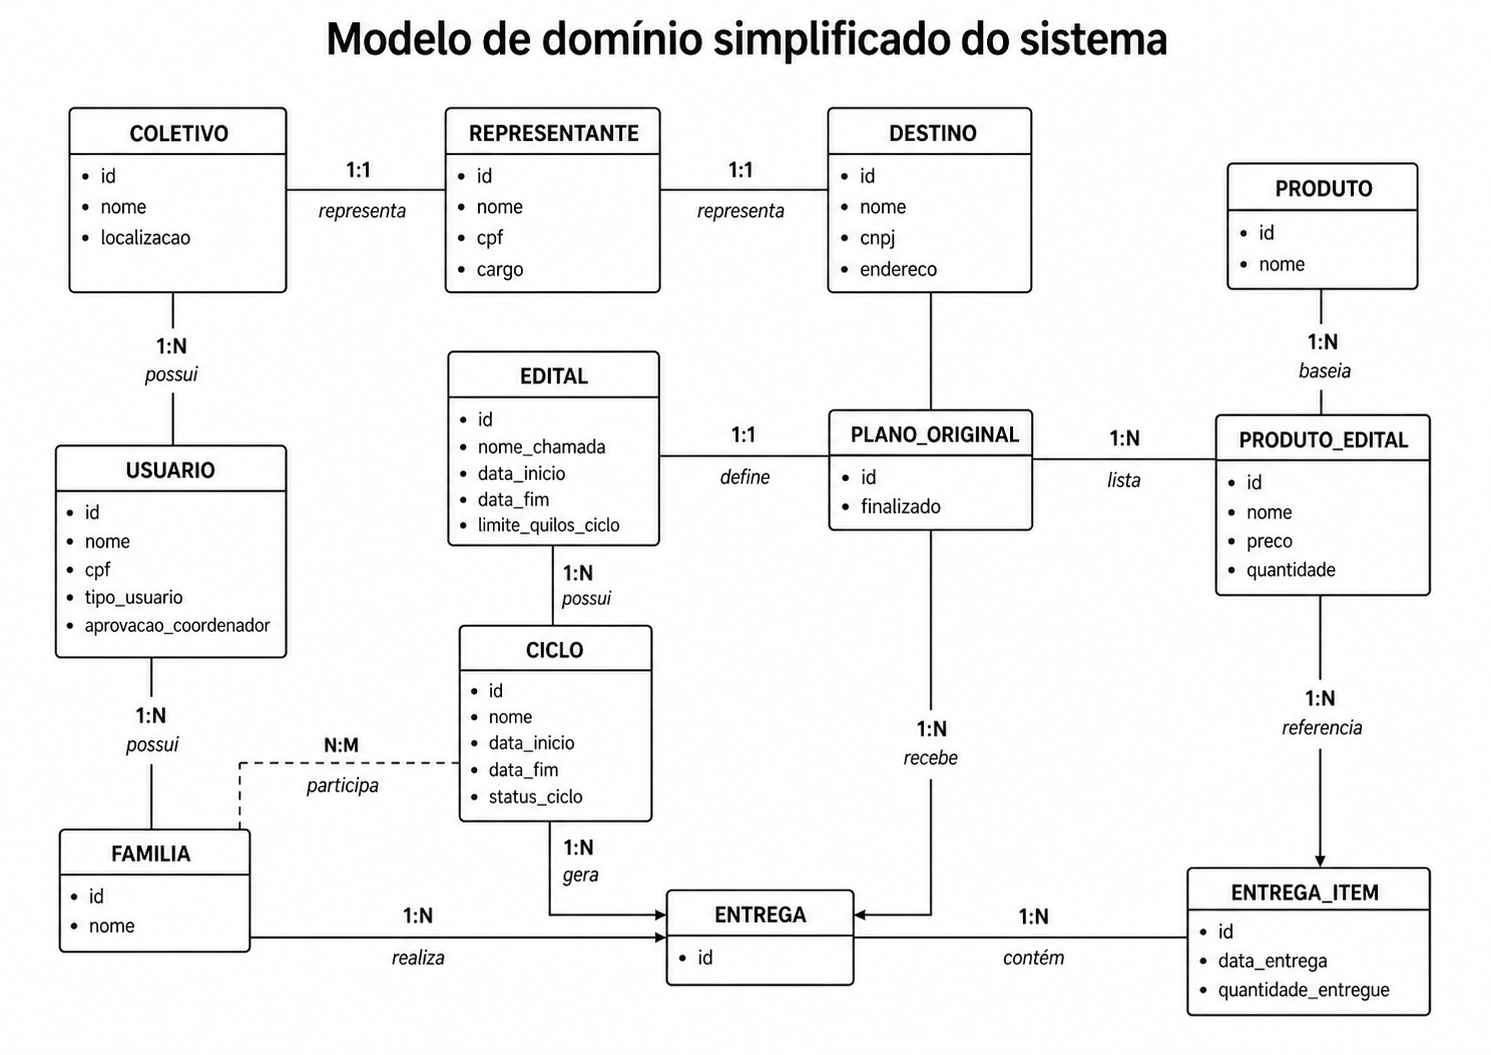
\includegraphics[width=1\textwidth]{Imagens/chap05/modelagem-diagrama-relacionamento.png}
    \caption{Modelo de domínio simplificado do sistema}
    \label{fig:modelo-dominio}
\end{figure}


\section{Arquitetura geral do sistema}

A arquitetura geral do sistema foi pensada para organizar o desenvolvimento em partes bem definidas, separando a interface utilizada pelos usuários das regras de negócio e do armazenamento das informações. Como o sistema precisa lidar com módulos e cada um com sua respectiva função, a aplicação foi estruturada para permitir que cada parte evolua de forma mais organizada, sem que uma alteração em uma funcionalidade comprometa todo o sistema.

O sistema foi desenvolvido como uma aplicação web, pois esse formato facilita o acesso por diferentes dispositivos, como computadores, notebooks e celulares.

Um ponto considerado na arquitetura foi a necessidade de manter o sistema preparado para novas funcionalidades, a arquitetura foi pensada de forma modular, permitindo que novos módulos sejam incorporados progressivamente, sem afetar o comportamento atual do sistema.

A estrutura geral é composta por duas partes principais: o frontend e o backend. O frontend é responsável pela interface com o usuário, apresentando as telas, formulários, tabelas e informações necessárias para a gestão do PAA. O backend é responsável por receber as requisições da interface, aplicar as regras de negócio e realizar a comunicação com o banco de dados. 

A intenção de manter o frontend e o backend separados era de dar independência ao desenvolvimento de cada um. Mesmo que um complete o outro, funcionalidades como filtros podem ser aplicadas ao backend sem que seja necessário derrubar toda a aplicação.

\section{Implementação do backend}

Seguindo princípios de arquitetura limpa, a estrutura de pastas do backend foi dividida em application, domain, infrastructure e web. A application é responsável pelas interfaces dos services que serão implementados. O domain representa todas as entidades do sistema que foram explicadas em seções anteriores, assim como DTOs e as interfaces que são implementadas em tempo de execução para o armazenamento no banco de dados. A infrastructure é responsável por armazenar configurações necessárias, a implementação dos services que dão a alma para o sistema e funções utilitárias para o sistema. A pasta web é responsável por armazenar os controllers que são o ponto de entrada das requisições, sejam elas vindas do frontend ou de alguma ferramenta que realiza requisições HTTP. A Figura~\ref{fig:directory-structure} ilustra a organização de diretórios do projeto.

\begin{figure}[H]
    \centering
    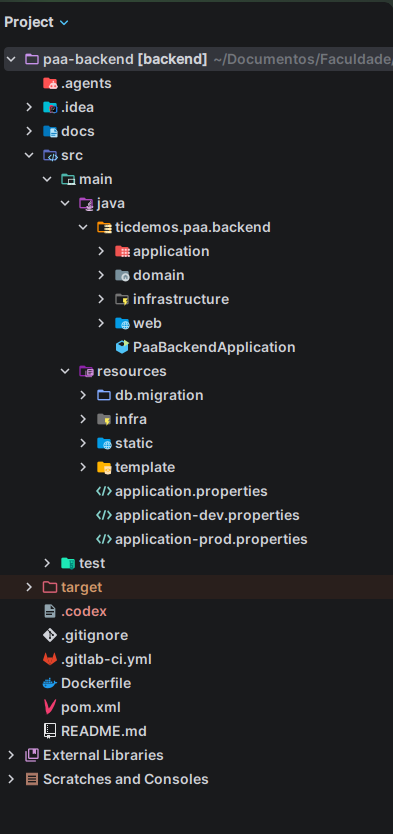
\includegraphics[width=0.5\textwidth]{Imagens/chap05/structure-directory.png}
    \caption{Estrutura de diretórios do backend}
    \label{fig:directory-structure}
\end{figure}

A tecnologia utilizada para implementar o backend foi o Java 17, juntamente com o framework Spring Boot 3. Essa escolha permitiu estruturar a aplicação de forma modular, facilitando a criação de APIs, a organização das regras de negócio e a integração com o banco de dados. Para a criação dos endpoints e dos controllers responsáveis por receber as requisições da interface, foi utilizado o Spring Web, que permitiu organizar as rotas HTTP utilizadas pelo frontend.

Para melhorar a experiência de desenvolvimento e simplificar a comunicação com o banco de dados, foi utilizado o Spring Data JPA em conjunto com o Hibernate, uma ferramenta de mapeamento objeto-relacional (ORM). Com o uso dessas tecnologias, as entidades do sistema podem ser representadas por classes Java, permitindo que operações de armazenamento e consulta sejam realizadas por meio de métodos e repositórios da aplicação. Dessa forma, reduz-se a necessidade de escrever comandos SQL diretamente.

O banco de dados escolhido foi o PostgreSQL, por ser uma ferramenta open-source, robusta e amplamente utilizada em aplicações web. Além disso, o PostgreSQL oferece bom desempenho tanto para sistemas em estágio inicial, como MVPs, quanto para aplicações maiores, que exigem maior consistência, confiabilidade e capacidade de expansão. Durante o desenvolvimento, o pgAdmin foi utilizado como ferramenta de apoio para visualizar tabelas, acompanhar registros e verificar informações armazenadas no banco de dados.

Para lidar com questões de segurança da aplicação, foi inserido no projeto o Spring Security, possibilitando o controle de acesso às rotas restritas e o bloqueio de endpoints para usuários não autenticados. Além disso, foi adotado o uso de JWT, permitindo que as requisições ao backend fossem realizadas de forma autenticada e associadas ao usuário logado. Com isso, tornou-se possível controlar o acesso às funcionalidades do sistema de acordo com o perfil de cada usuário.

Para os testes unitários, foram utilizadas as bibliotecas JUnit e Mockito. O JUnit permite estruturar e executar os testes automatizados, enquanto o Mockito possibilita simular comportamentos de componentes da aplicação, como serviços e repositórios. Essas ferramentas contribuem para validar processos críticos, como criação, atualização e consulta de dados, além de ajudar a garantir que mudanças futuras no código não comprometam comportamentos já implementados. O gerenciamento das dependências, a execução dos testes e a geração do pacote da aplicação foram organizados por meio do Maven, mantendo uma estrutura padronizada para o projeto backend.

Na documentação da API, foi utilizado o OpenAPI/Swagger, por ser uma ferramenta open-source que gera uma interface interativa para visualização e teste dos endpoints da aplicação. Com isso, torna-se possível consultar os recursos disponíveis, verificar os parâmetros esperados e testar requisições diretamente pela própria aplicação, sem a necessidade inicial de ferramentas externas. 

\section{Implementação do frontend}

O frontend foi pensado para tornar o sistema intuitivo e facilitar o uso pelos diferentes perfis de usuários. No caso do coordenador e do administrador, a interface busca auxiliar na administração dos editais do PAA. Já para o agricultor, o objetivo é permitir o acompanhamento claro do andamento de sua participação no edital.

No desenvolvimento das telas e dos componentes do sistema, foi utilizada a biblioteca React 19. Para personalizar a interface e aproximar o projeto dos padrões visuais presentes em aplicações web atuais, foi escolhida a biblioteca MUI. Além de ser open-source, essa biblioteca implementa os princípios do Material Design, proposto pelo Google, contribuindo para a construção de uma interface padronizada, responsiva e de fácil utilização. A estilização dos componentes também utiliza o Emotion, tecnologia associada ao ecossistema do MUI e utilizada para organizar estilos aplicados à interface.

O TypeScript está presente em todo o desenvolvimento do frontend, pois contribui para manter maior coerência entre os dados manipulados pela aplicação. Como o sistema realiza troca constante de informações com o backend, os dados recebidos e enviados são tipados, o que reduz erros durante o desenvolvimento e facilita a manutenção do código.

Além da biblioteca de design, o frontend utiliza outras ferramentas importantes para a organização da aplicação. O roteamento das páginas é realizado com o React Router DOM, permitindo controlar a navegação entre as diferentes telas do sistema. Para o gerenciamento de estado, são utilizados o Redux Toolkit e o React Redux, que centralizam o estado da aplicação em uma store e organizam as alterações por meio de actions e reducers. Essa abordagem contribui para tornar o comportamento da interface mais previsível, principalmente em telas que dependem de dados compartilhados entre diferentes componentes.

A comunicação com o backend é feita por meio da biblioteca Axios, responsável por realizar requisições HTTP para a API do sistema. Também são utilizadas bibliotecas auxiliares para formatação e processamento de datas, contribuindo para a apresentação adequada das informações ao usuário. O Vite foi utilizado como ferramenta de desenvolvimento e construção do frontend, facilitando a execução local da aplicação e a geração dos arquivos de produção. Além disso, o ESLint foi utilizado para auxiliar na padronização do código e na identificação de problemas durante o desenvolvimento. Todas as bibliotecas utilizadas no frontend são gerenciadas pelo arquivo package.json, por meio do npm, que organiza as dependências necessárias para o funcionamento e a manutenção da aplicação.

\subsection{Telas implementadas}

A seguir, são apresentadas as telas do sistema, juntamente com a descrição de cada uma. A Figura~\ref{fig:login} mostra a primeira tela, a de login, na qual os usuários já cadastrados podem inserir suas credenciais e acessar o sistema, enquanto os interessados podem solicitar acesso por meio do botão de criação de conta.


\begin{figure}[H]
    \centering
    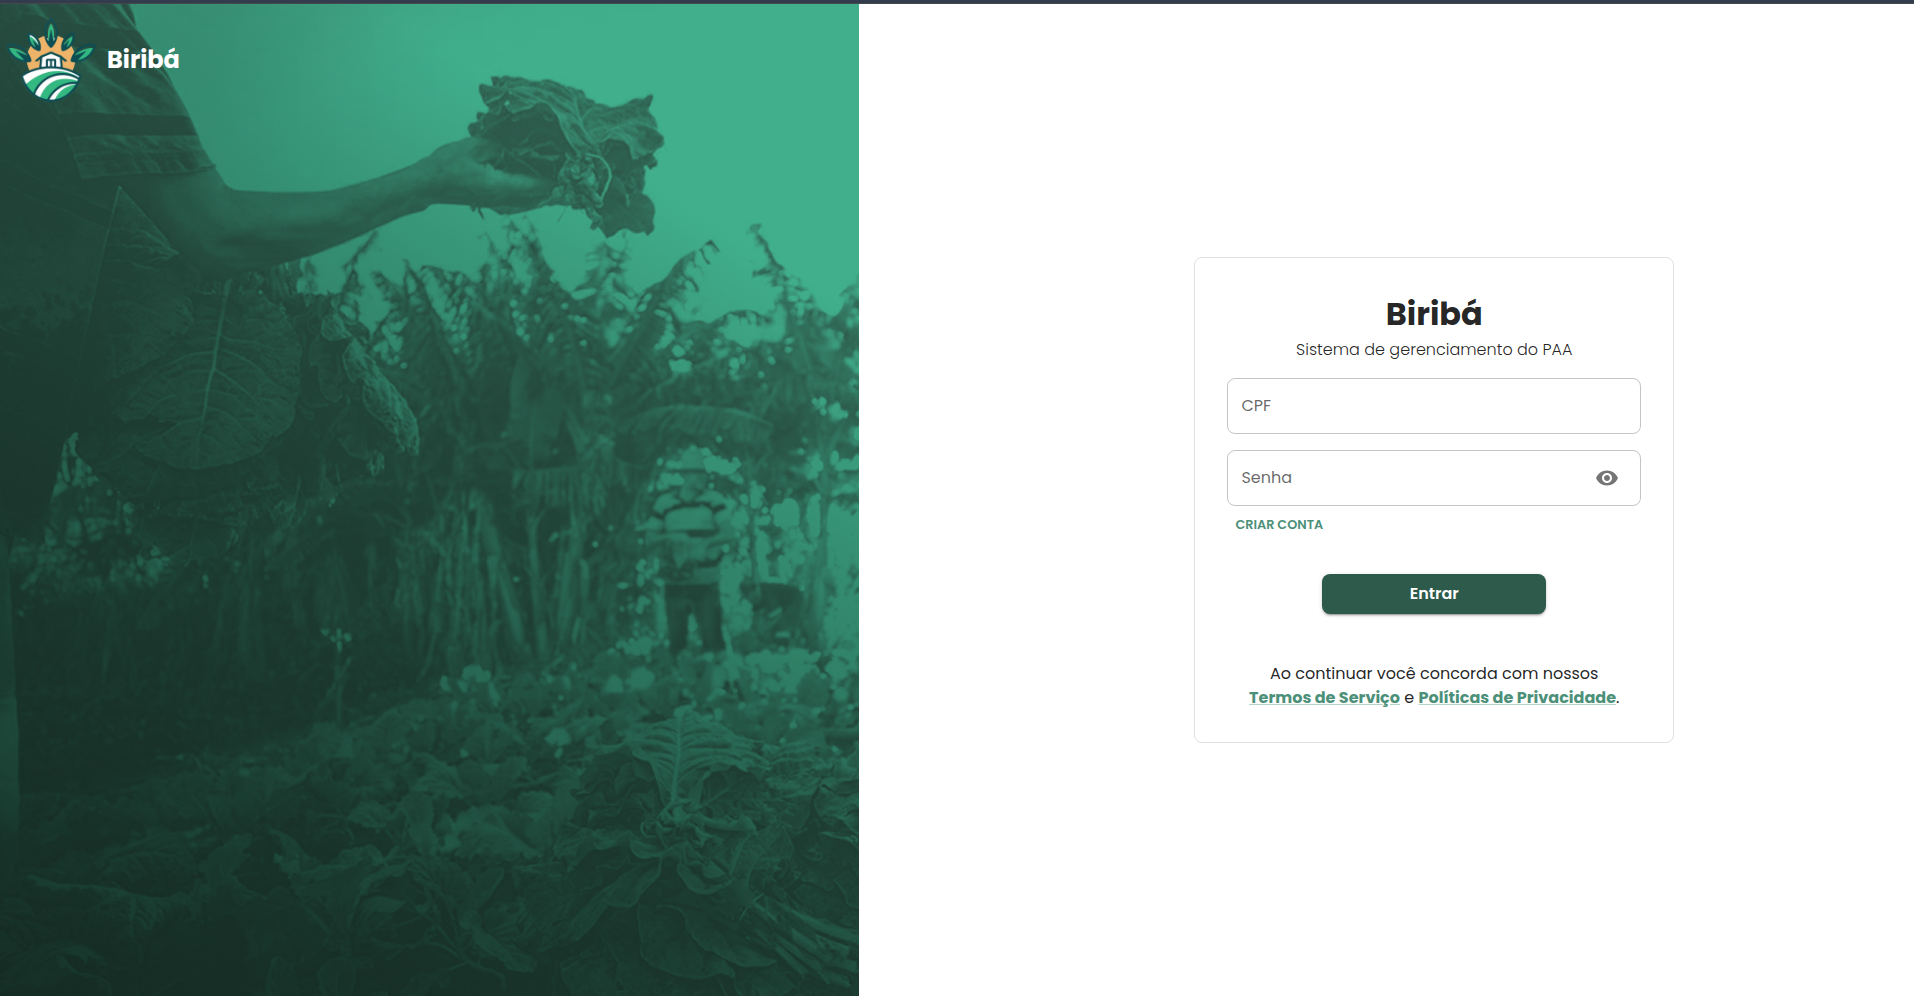
\includegraphics[width=1\textwidth]{Imagens/chap05/login_biriba.png}
    \caption{Login do sistema}
    \label{fig:login}
\end{figure}

Após o login, o usuário segue para a seleção do edital cujo andamento deseja verificar ou cujo gerenciamento pretende realizar. A tela apresentada na Figura~\ref{fig:editais} exibe todos os editais disponíveis para seleção. Vale ressaltar que o coordenador só pode acompanhar o andamento dos editais de seu coletivo. Um filtro é realizado no backend para que os dados exibidos na interface sigam essa regra. O administrador do sistema pode visualizar todos os editais existentes, enquanto o agricultor possui acesso semelhante ao do coordenador e pode visualizar somente os editais dos quais participa. A tela também apresenta um botão para a criação de novos editais, permitindo que o coordenador ou o administrador inicie o gerenciamento de uma nova chamada pública.

\begin{figure}[H]
    \centering
    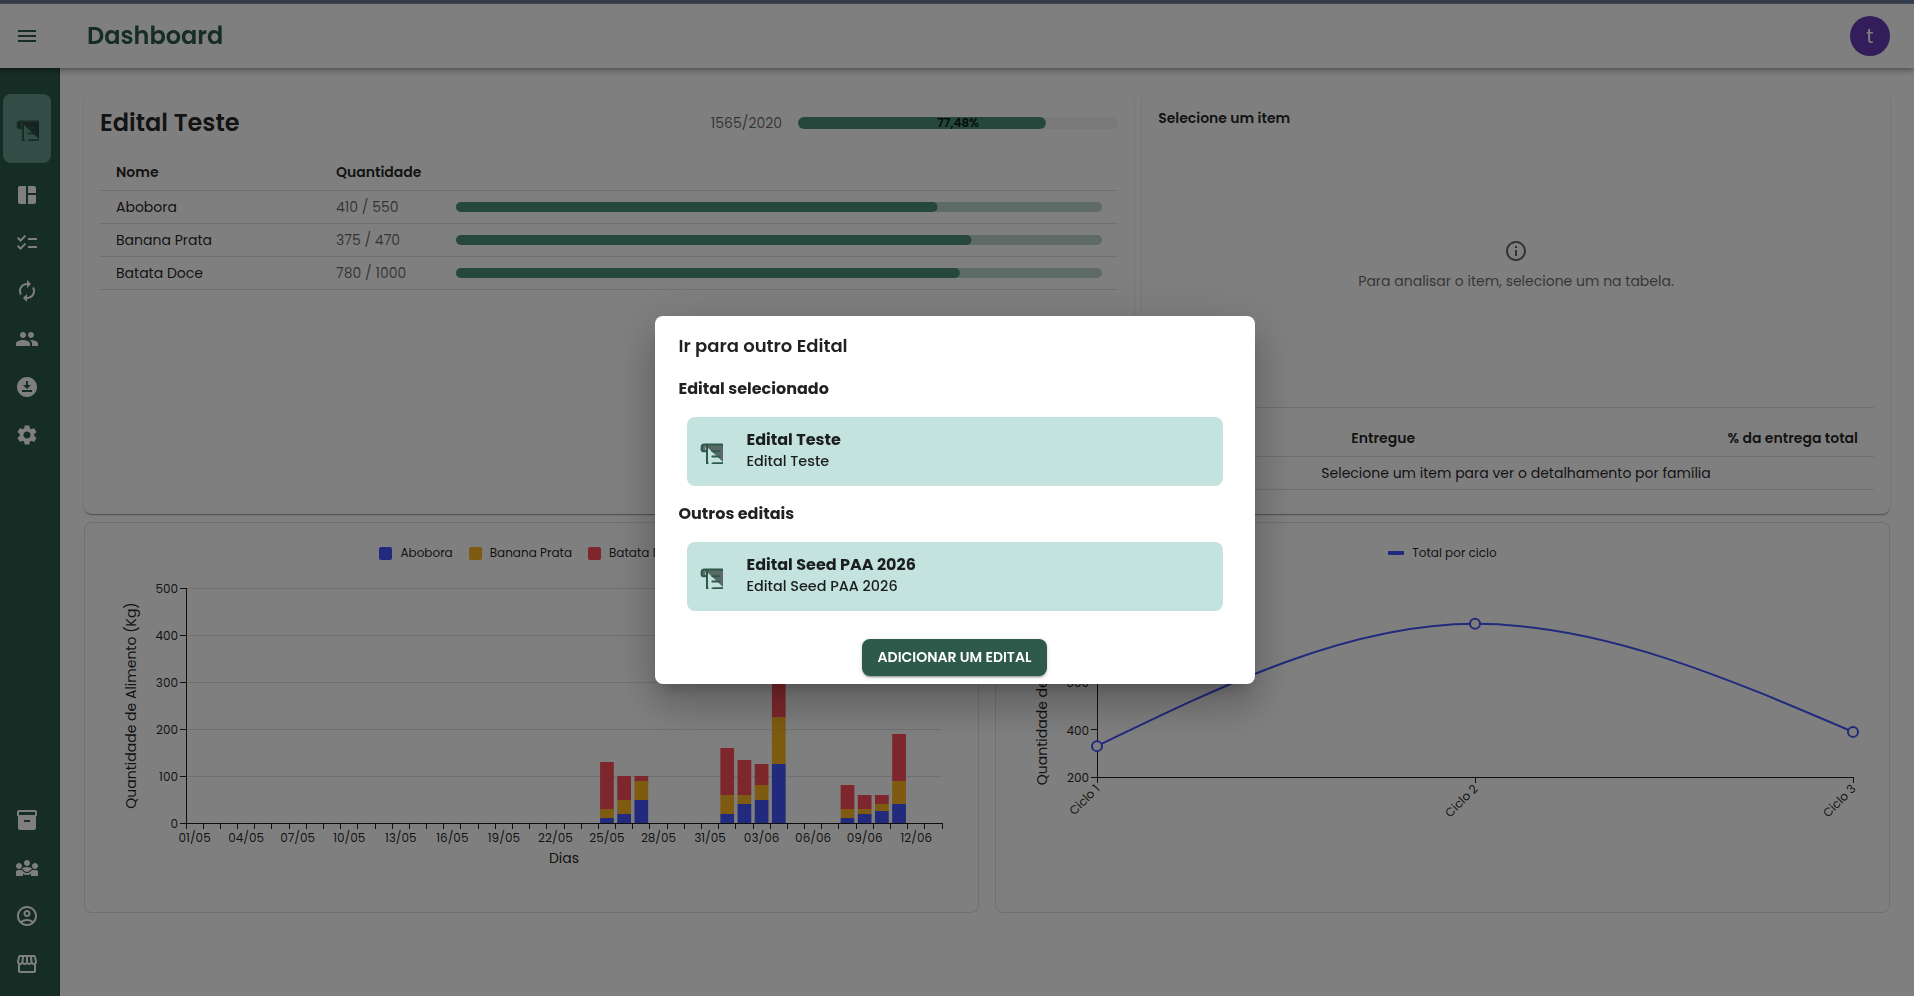
\includegraphics[width=1\textwidth]{Imagens/chap05/selecao_edital.png}
    \caption{Seleção de editais}
    \label{fig:editais}
\end{figure}

Em seguida, na criação do edital, o coordenador deverá preencher o plano original, definindo quais famílias participarão do edital, quais produtos serão ofertados e quais serão os destinos das entregas. A Figura~\ref{fig:plano-original-vazio} exemplifica um plano original parcialmente preenchido, contendo apenas as famílias e os produtos. Nessa mesma figura, observa-se a presença de botões para adicionar uma nova família ao edital e para incluir um novo produto.

Na Figura~\ref{fig:plano-original-preenchido}, é apresentada a aba de produtos por família já preenchida no plano original. A primeira coluna da tabela corresponde aos produtos que farão parte do edital selecionado, enquanto a segunda coluna indica o valor do quilo de cada produto. As demais colunas, com exceção da última, representam as famílias participantes do edital.

Em cada linha, as células associadas às famílias indicam a quantidade de determinado produto que cada família deverá entregar ao longo do edital. A última coluna apresenta o valor total, em reais, correspondente à quantidade total prevista para aquele produto. Já a última célula de cada coluna referente às famílias mostra o valor total que cada família deverá receber ao final do edital. Por fim, a célula localizada na última linha e na última coluna da tabela apresenta o valor total previsto para o edital, considerando todos os produtos e todas as famílias participantes.

Na Figura~\ref{fig:plano-original-destino}, é apresentado um exemplo de preenchimento da aba de produtos por destino. Essa tabela possui estrutura semelhante à aba anterior, mas, nesse caso, as colunas representam os destinos das entregas. Cada célula das colunas de destino indica a quantidade de determinado produto que será enviada para aquele destino ao longo do edital.

A última coluna dessa tabela é utilizada como referência para orientar o coordenador na distribuição dos produtos entre os destinos. Ela é preenchida a partir das quantidades previamente definidas para os agricultores na aba de produtos por família, permitindo verificar quanto de cada produto ainda precisa ser distribuído. Dessa forma, o coordenador consegue organizar a destinação dos alimentos de acordo com o total previsto no plano original.

Na página do plano original, além dos botões para adicionar produtos, famílias e destinos, há também o botão “Finalizar Plano Original”. Esse botão tem como objetivo encerrar a etapa de edição das tabelas e dar início ao andamento do edital. Após a finalização, as tabelas deixam de permitir alterações, garantindo que os dados definidos no plano original sejam preservados durante a execução do edital.

Observa-se que, nas Figuras~\ref{fig:plano-original-preenchido} e~\ref{fig:plano-original-destino-completo}, esse botão aparece desabilitado, e os botões de inclusão não estão presentes na tela. Isso indica que o plano original já foi finalizado e que a edição das informações foi bloqueada.


\begin{figure}[H]
    \centering
    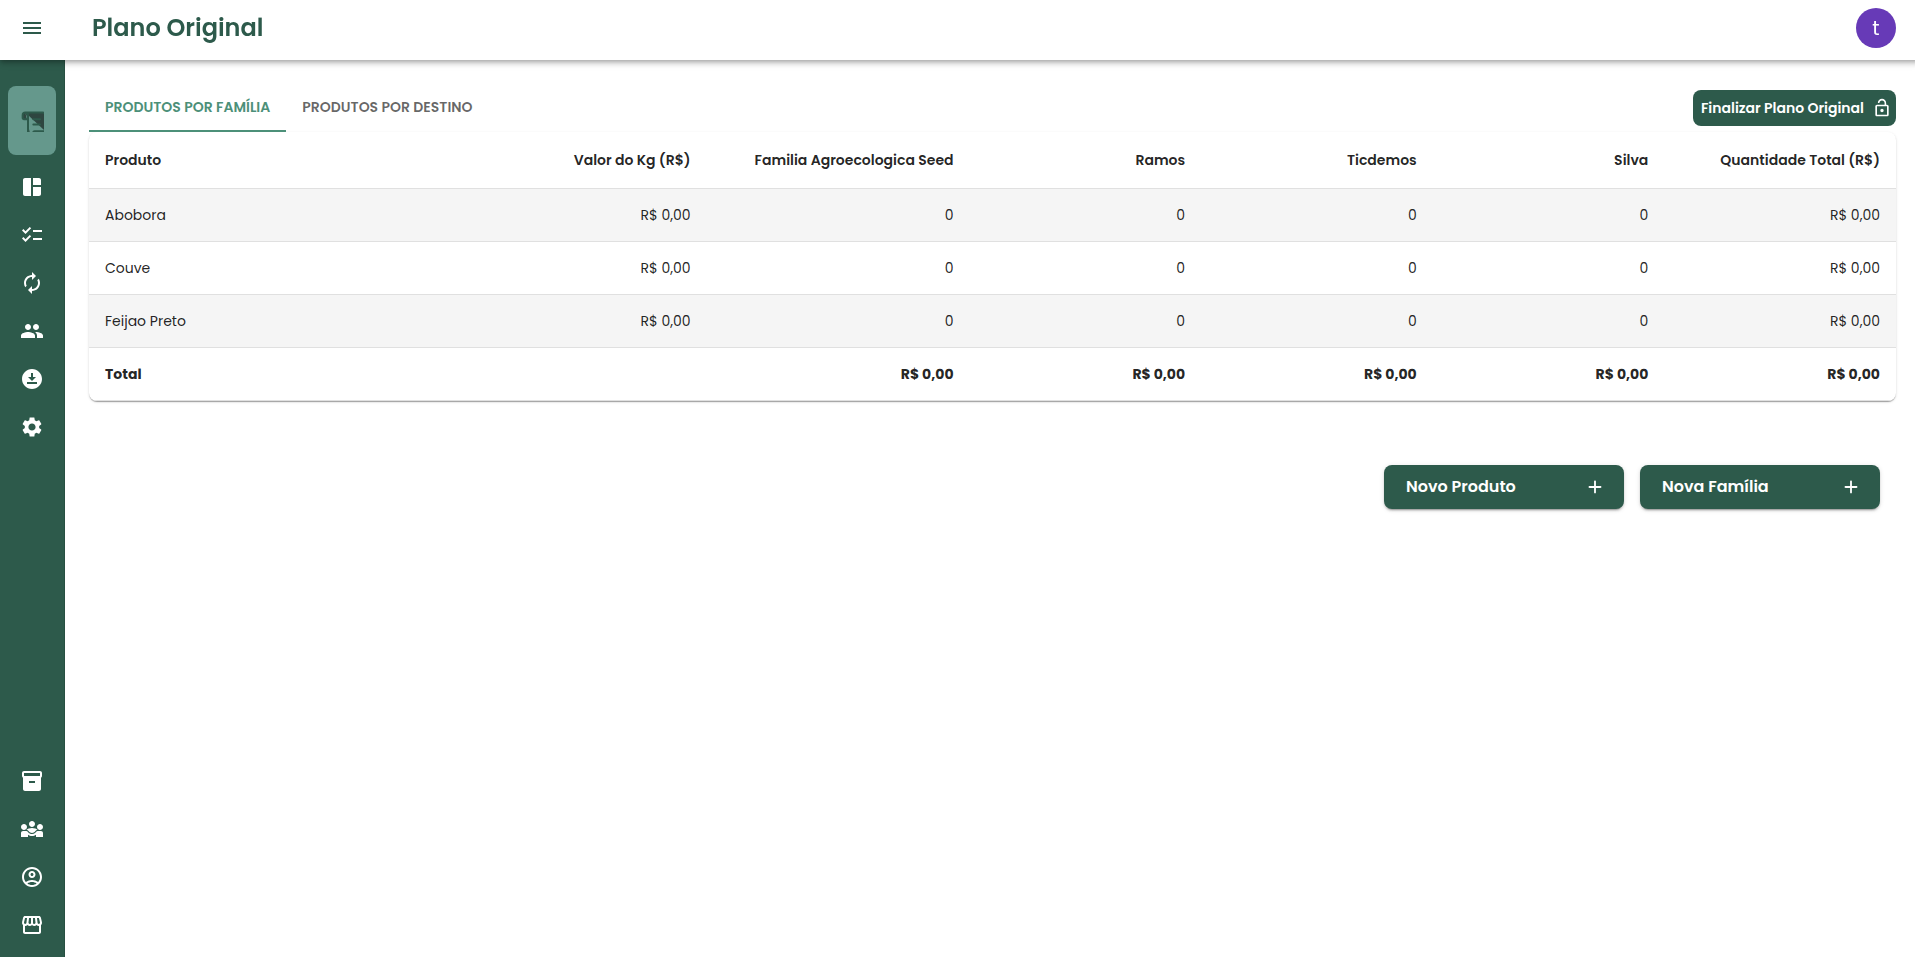
\includegraphics[width=1\textwidth]{Imagens/chap05/plano_original_vazio.png}
    \caption{Plano original aba produto por família parcialmente preenchido}
    \label{fig:plano-original-vazio}
\end{figure}

\begin{figure}[H]
    \centering
    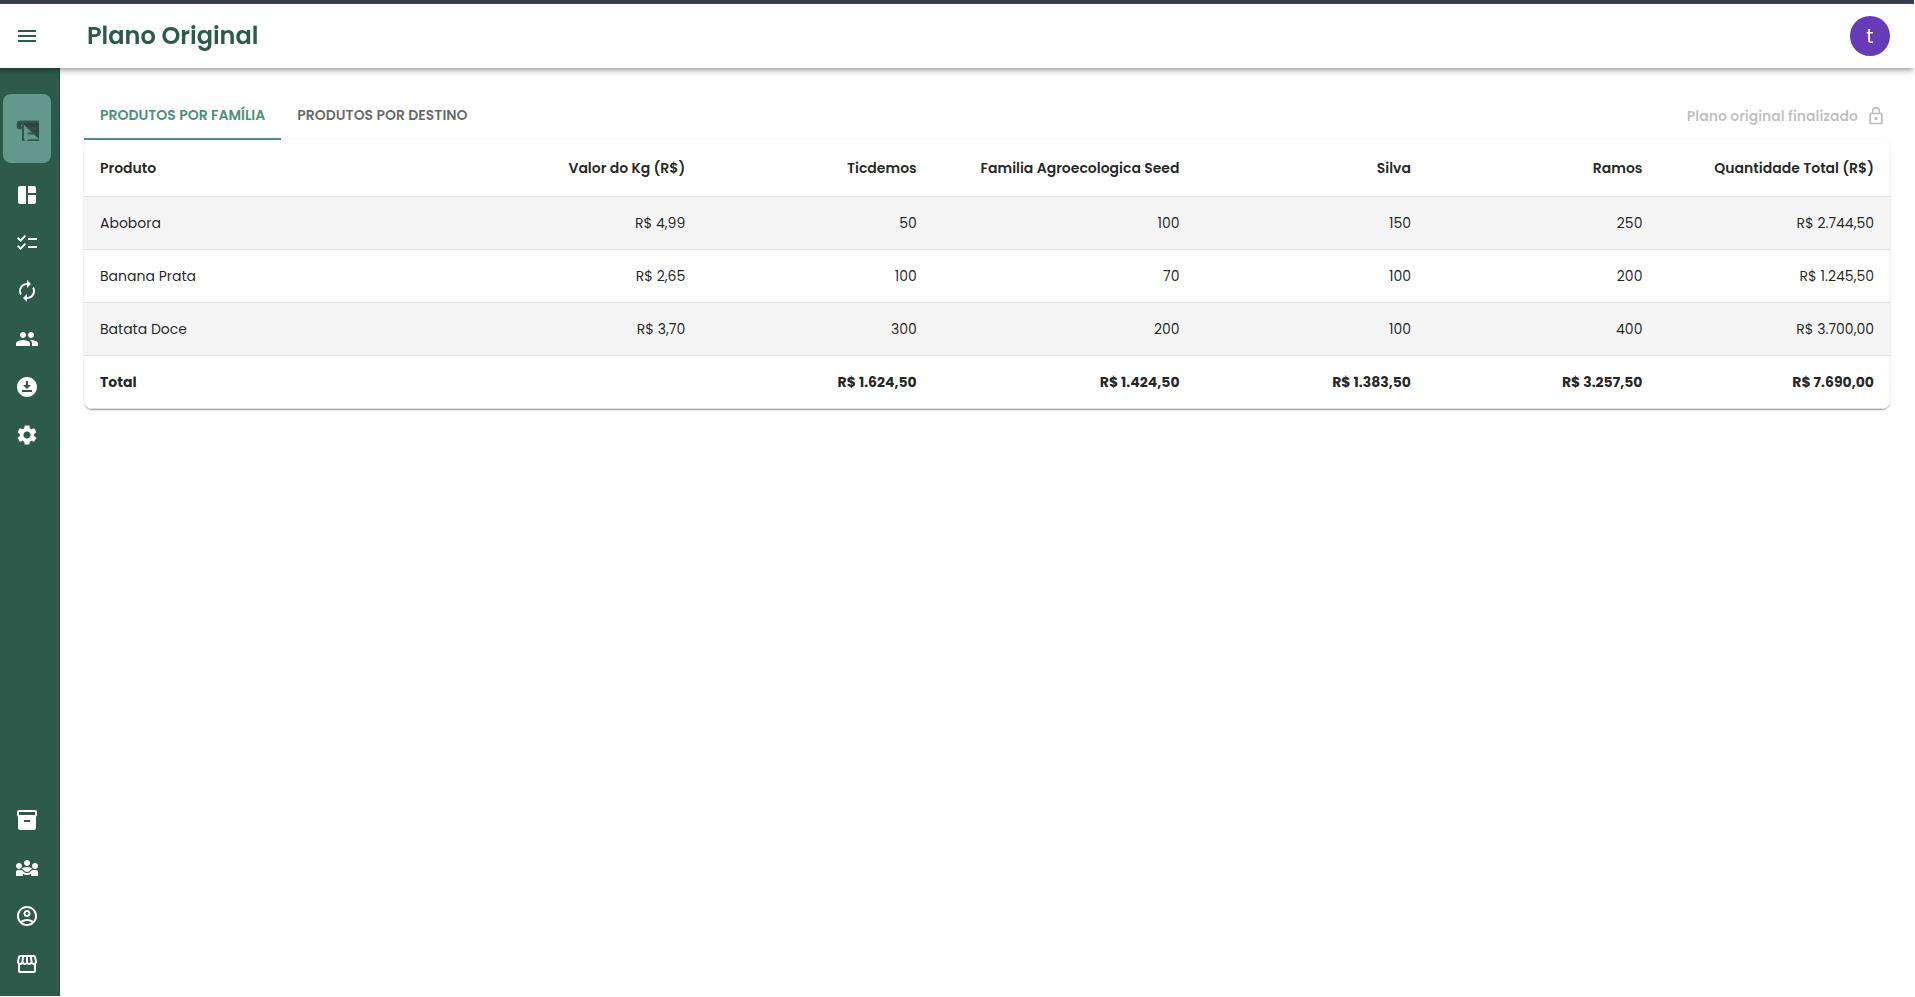
\includegraphics[width=1\textwidth]{Imagens/chap05/tela_plano_original.png}
    \caption{Plano original aba produto por família completo}
    \label{fig:plano-original-preenchido}
\end{figure}

\begin{figure}[H]
    \centering
    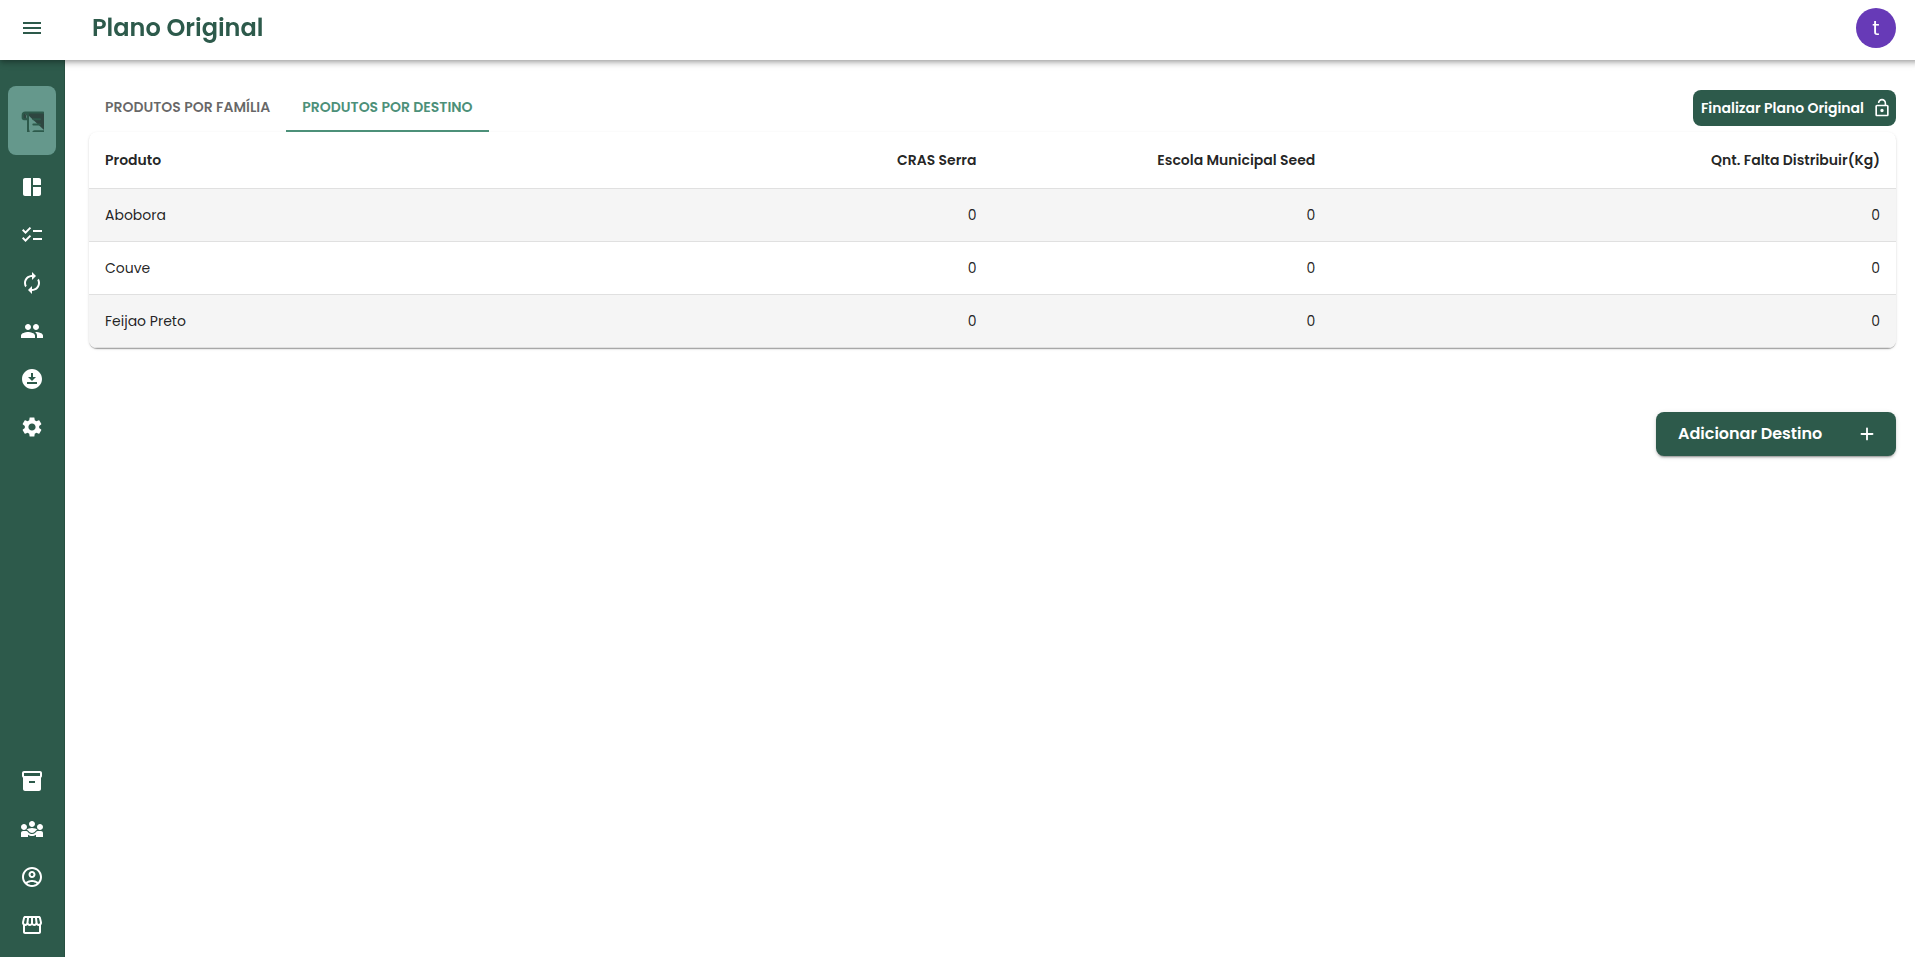
\includegraphics[width=1\textwidth]{Imagens/chap05/destino-semi-preenchido.png}
    \caption{Plano original aba produto por destino parcialmente preenchido}
    \label{fig:plano-original-destino}
\end{figure}

 \begin{figure}[H]
    \centering
    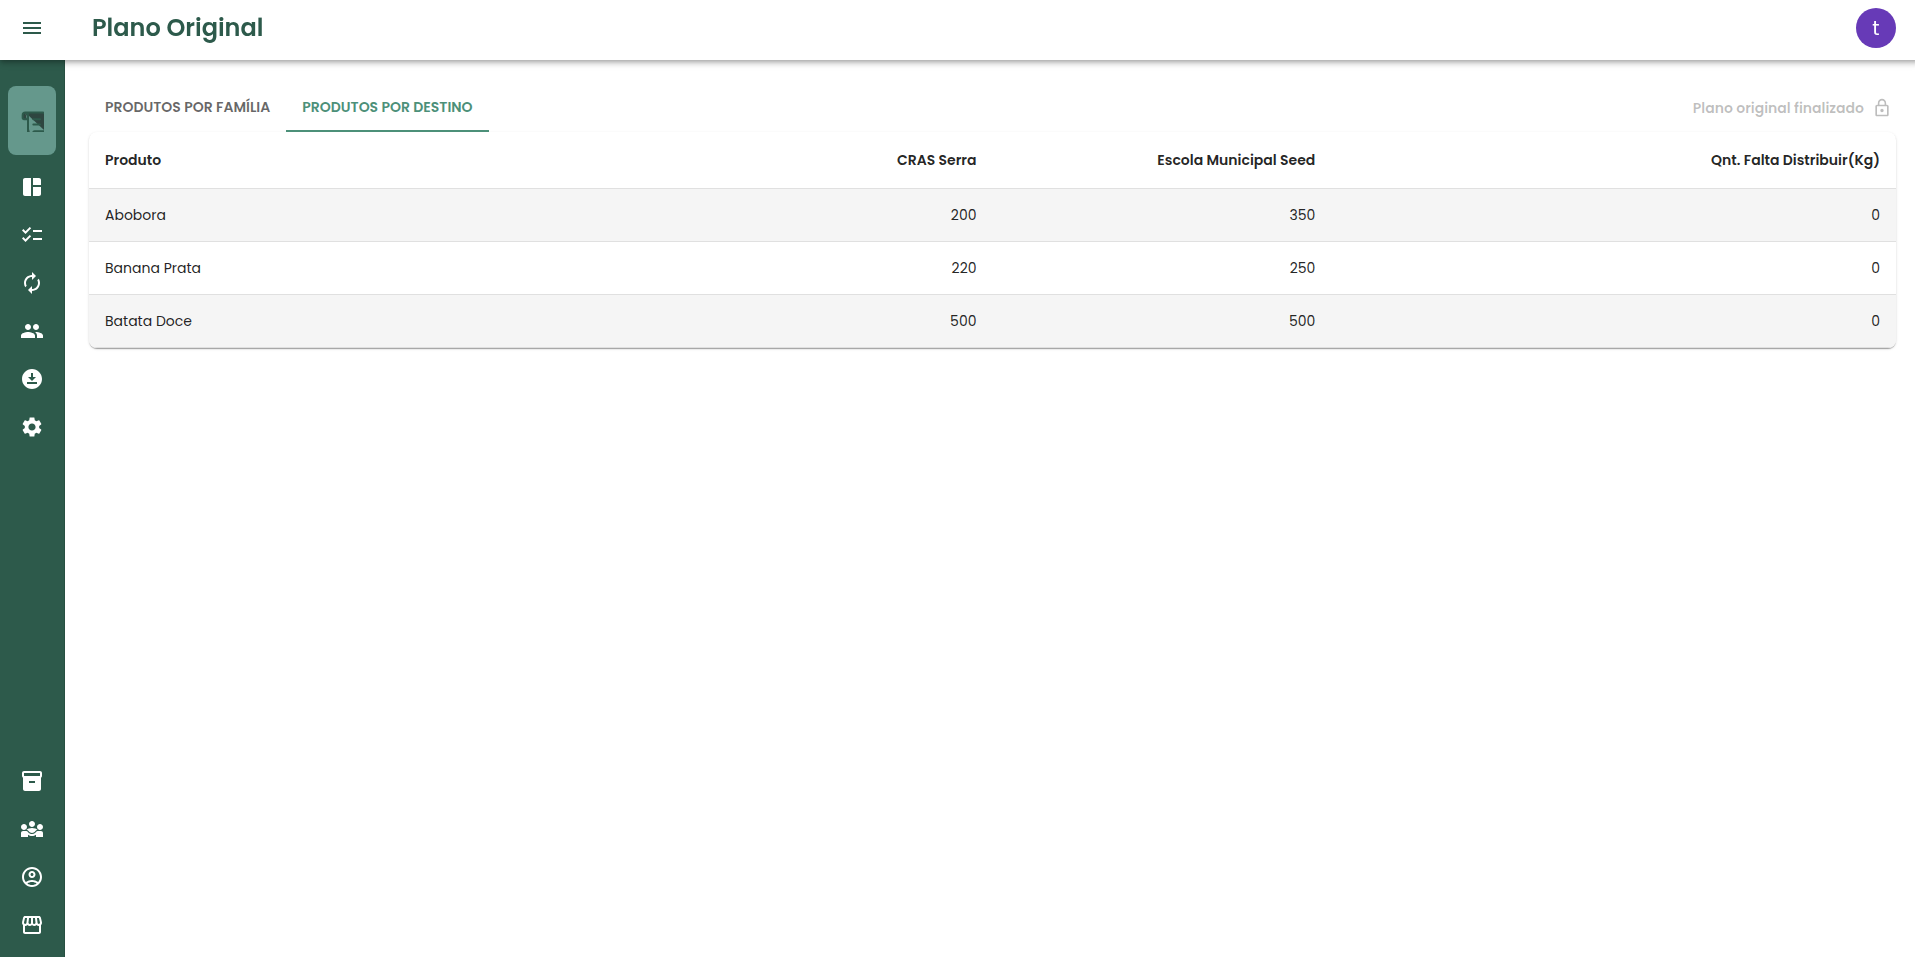
\includegraphics[width=1\textwidth]{Imagens/chap05/destino_plano_orignal.png}
    \caption{Plano original aba produto por destino completo}
    \label{fig:plano-original-destino-completo}
\end{figure}

Após a finalização do plano original, inicia-se a etapa de acompanhamento do andamento do edital por meio da tela de ciclos de entrega. Nessa tela, o coordenador pode criar os ciclos, definindo suas datas de início e fim, além de registrar a quantidade de produtos entregue por cada família e a quantidade destinada a cada local de entrega.

A Figura~\ref{fig:ciclo-entrega} exemplifica os três status possíveis dos ciclos já criados. Nessa tela, observa-se também a existência de dois controles principais: um relacionado às famílias e outro aos destinos. No controle de famílias, o coordenador registra as entregas realizadas em cada ciclo, informando a quantidade de produtos entregue por cada família. Para auxiliar esse processo, a tabela apresenta uma coluna de apoio que indica a quantidade ainda faltante de cada produto, considerando os valores definidos previamente no plano original.

O controle de destinos possui funcionamento semelhante. Nele, o coordenador define a quantidade de produtos que será encaminhada para cada destino em determinado ciclo. Ao lado das informações de entrega, o sistema apresenta a quantidade total prevista para cada destino ao longo do edital, permitindo acompanhar se a distribuição está de acordo com o plano original. Além disso, ao lado do nome de cada destino, há um botão para baixar o relatório necessário à comprovação da entrega daquele ciclo.

Assim como ocorre na página do plano original, o ciclo de entrega pode ser finalizado antes da data prevista para o seu encerramento. Ao finalizar um ciclo, seu status é alterado e a edição das informações passa a ser bloqueada, garantindo maior controle sobre os dados registrados. No entanto, diferentemente do plano original, um ciclo finalizado pode ser reaberto, caso seja necessário corrigir ou complementar alguma informação posteriormente.


\begin{figure}[H]
    \centering
    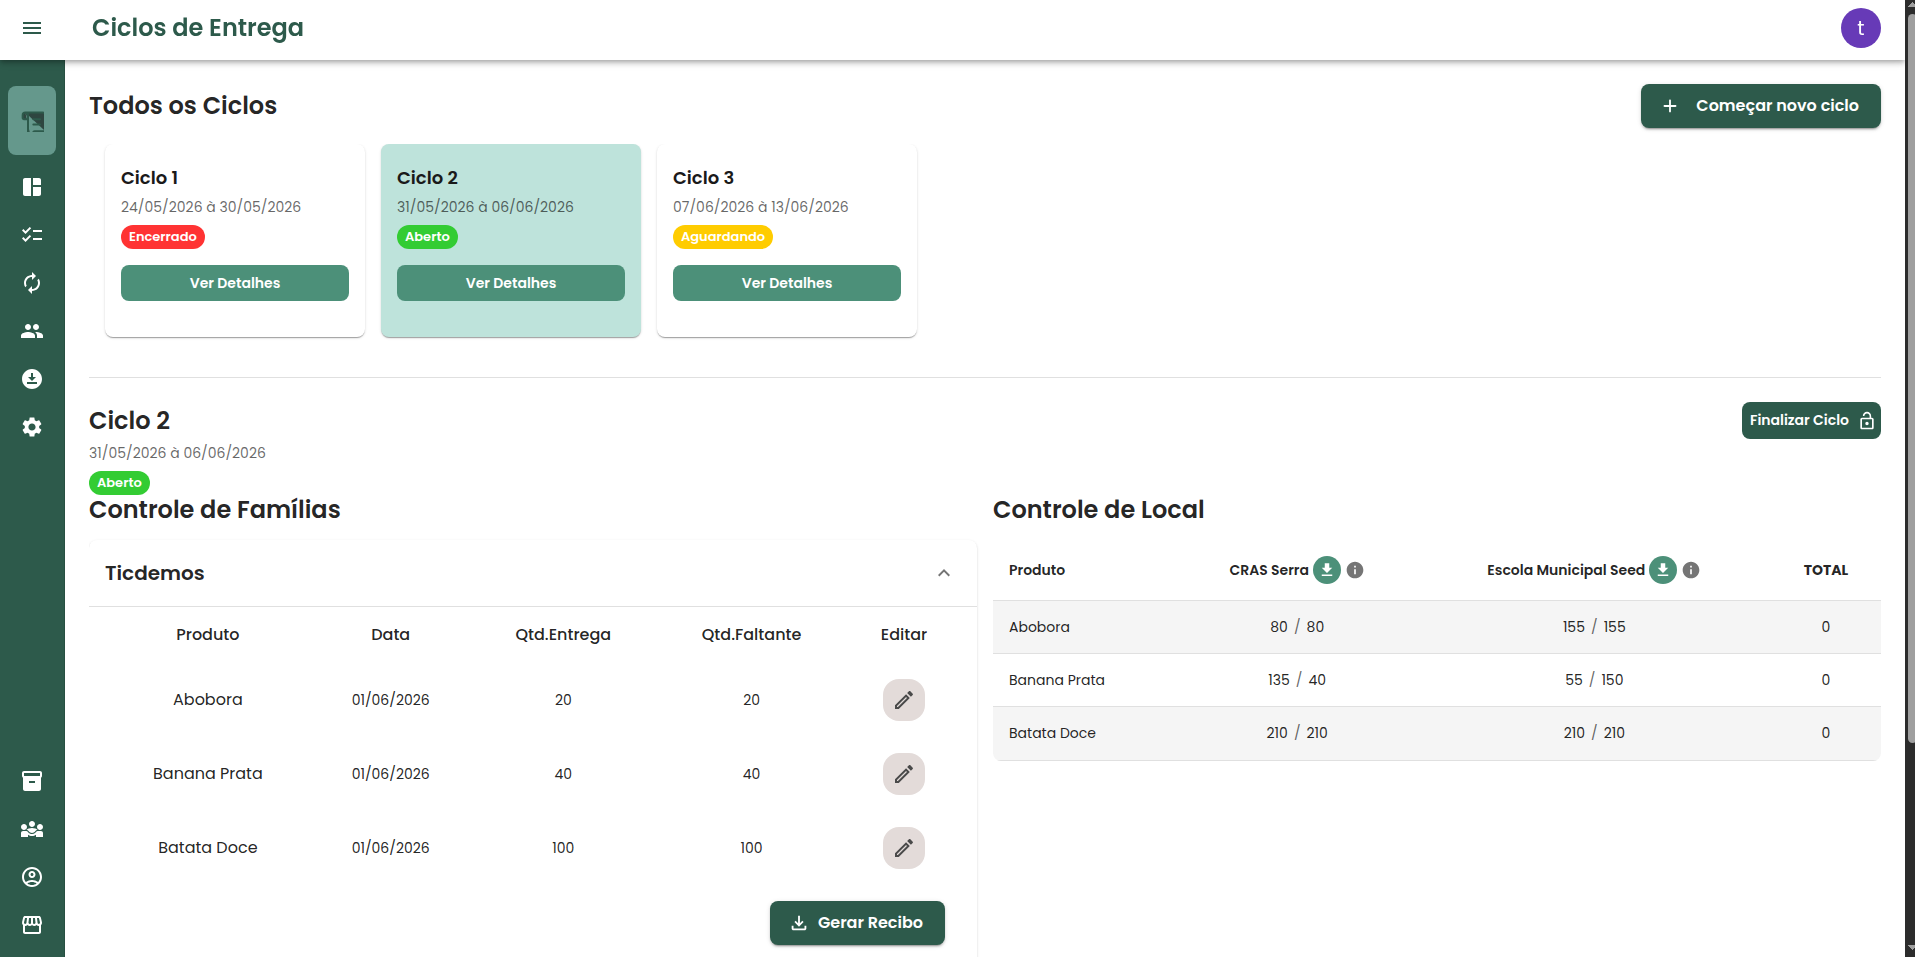
\includegraphics[width=1\textwidth]{Imagens/chap05/tela_ciclos_entrega.png}
    \caption{Ciclos e Entregas}
    \label{fig:ciclo-entrega}
\end{figure}


Após a finalização do ciclo de entrega, o coordenador pode baixar os relatórios referentes àquele período para cada destino. A Figura~\ref{fig:relatorios} apresenta, por meio de cards, todos os destinos vinculados ao edital, juntamente com suas principais informações. Em cada card, é possível baixar o relatório de recebimento de alimentos, utilizado para comprovar as entregas realizadas naquele destino. Dessa forma, os documentos são gerados pelo coordenador, mas registram informações que servem como comprovação das entregas feitas pelas famílias agricultoras.

Além disso, nessa mesma tela, há o botão para baixar o relatório de pagamento. Esse relatório sintetiza as entregas realizadas por família, apresentando a quantidade entregue e o valor que cada uma deverá receber ao final do ciclo.


\begin{figure}[H]
    \centering
    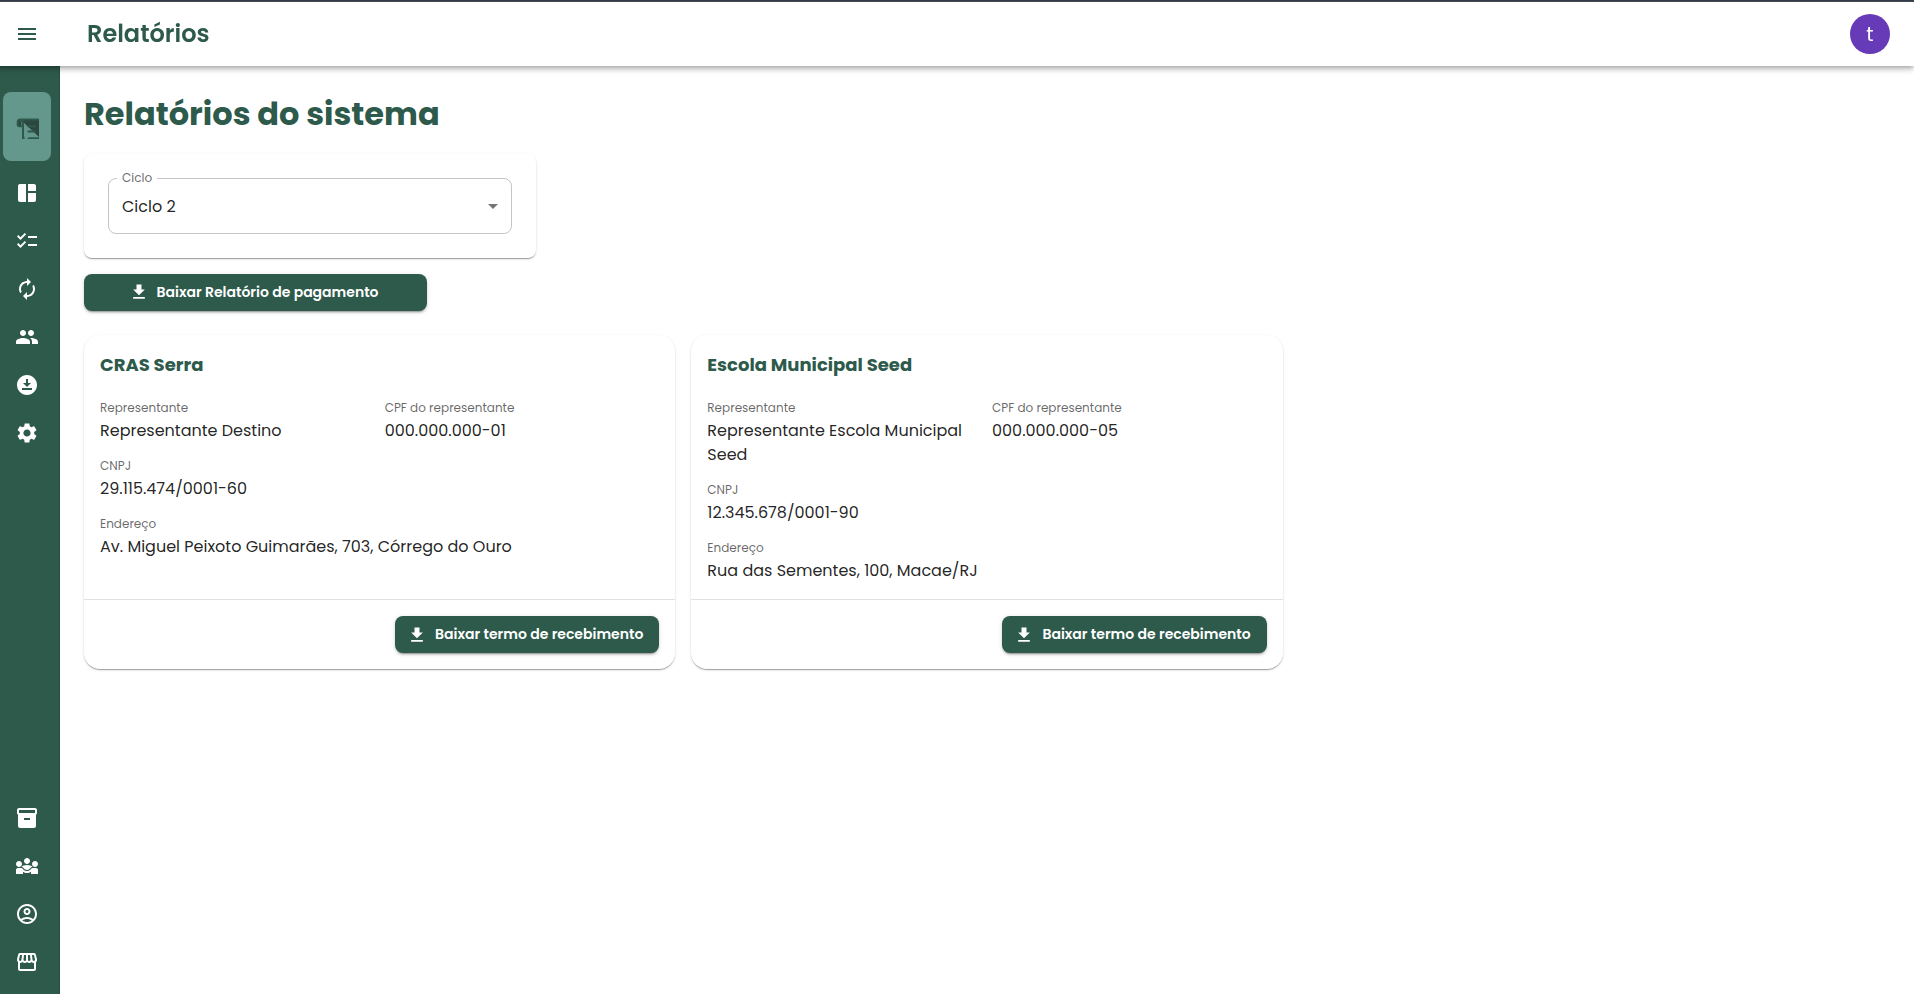
\includegraphics[width=1\textwidth]{Imagens/chap05/tela_relatorios.png}
    \caption{Relatórios}
    \label{fig:relatorios}
\end{figure}

Com o objetivo de permitir o acompanhamento individual de cada família, o coordenador tem acesso à tela de detalhes da família. Nessa tela, os dados dos ciclos de entrega são organizados por família, permitindo visualizar quanto foi entregue em cada ciclo e o valor total recebido. Além disso, o sistema possibilita a geração do recibo referente àquele ciclo para a família selecionada.

Na última coluna da tabela, há um recurso de apoio ao coordenador, que apresenta o acompanhamento acumulado das entregas ao longo dos ciclos. Essa coluna indica a quantidade de alimentos já entregue pela família e a quantidade ainda faltante em relação ao que foi definido no plano original. Na última célula da tabela, são apresentados o valor já recebido pela família e o valor que ainda deverá ser recebido até o final do edital. Abaixo, na Figura~\ref{fig:detalhes-familia} segue um exemplo.

\begin{figure}[H]
    \centering
    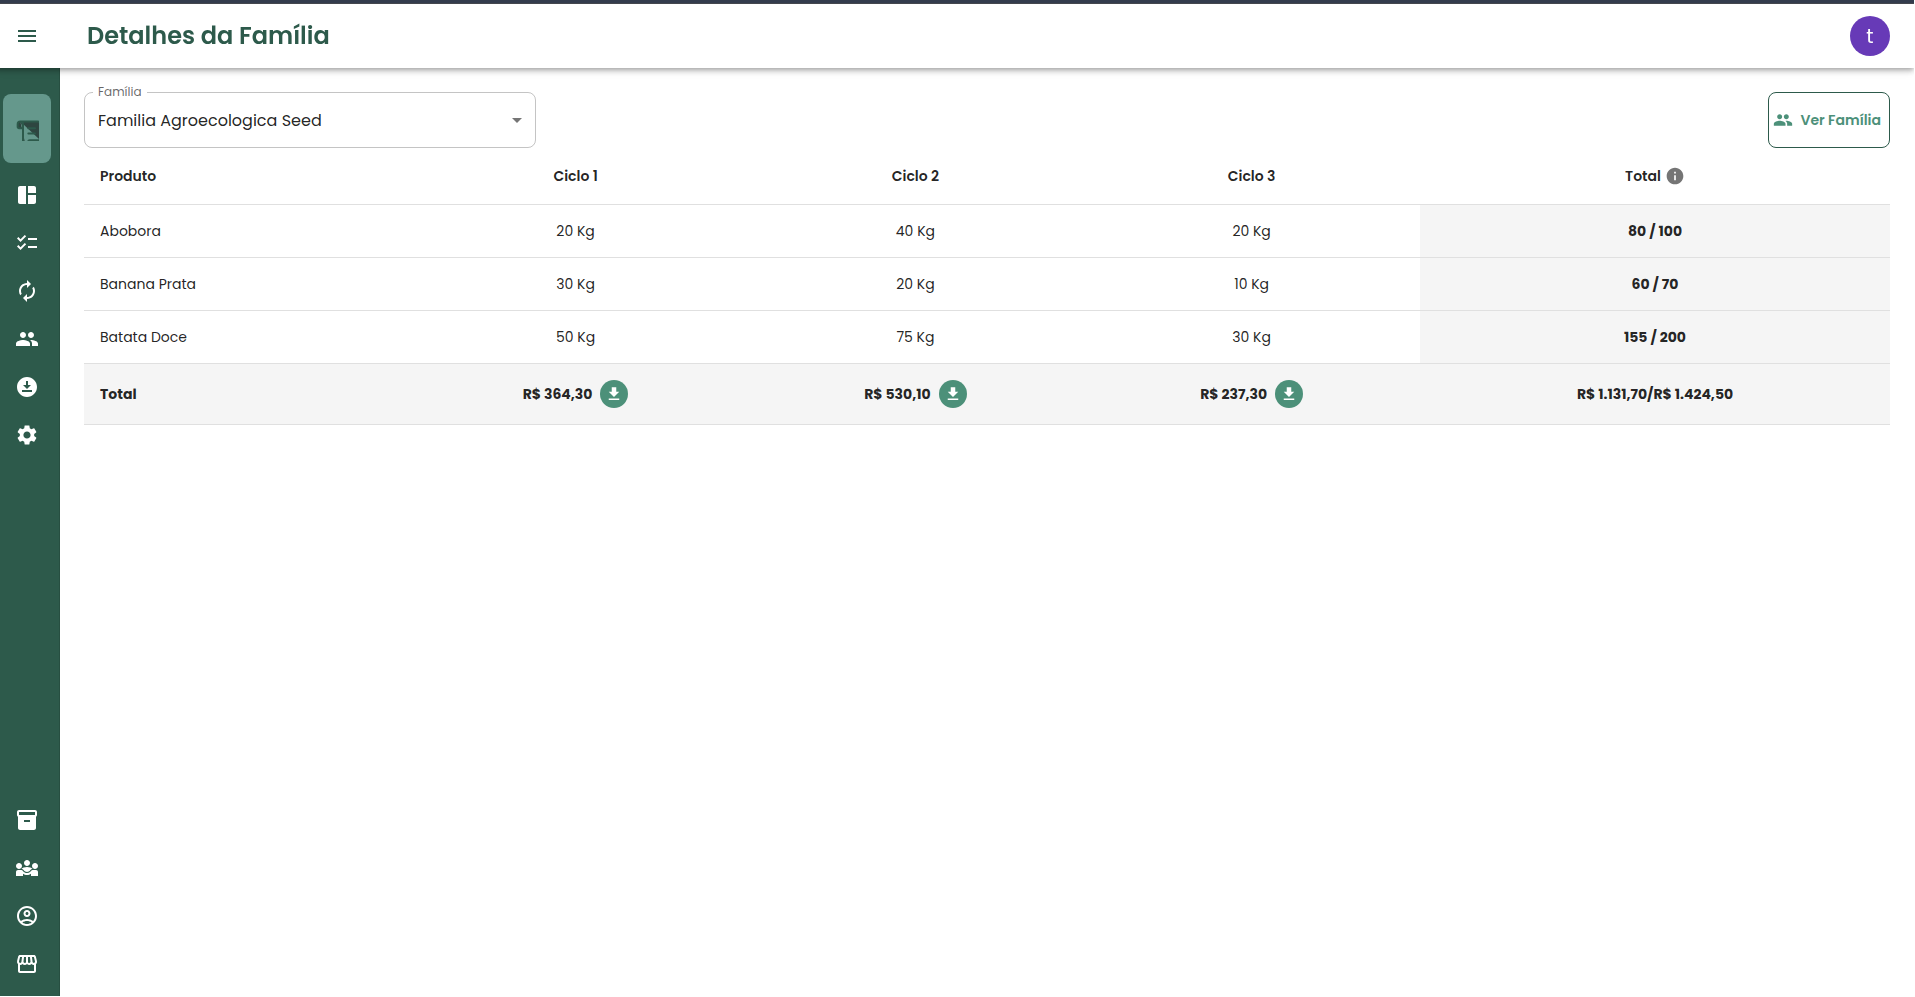
\includegraphics[width=1\textwidth]{Imagens/chap05/tela_detalhes_familia.png}
    \caption{Detalhes da família}
    \label{fig:detalhes-familia}
\end{figure}

Para verificar informações gerais do edital, o sistema possui a tela de configuração, onde há um resumo do cadastro inicial, com informações de início e fim, assim como a quantidade limite de quilos de alimento por entrega e por fim, um card que ao ser clicado redireciona para o plano original. Abaixo segue a imagem com exemplo.

\begin{figure}[H]
    \centering
    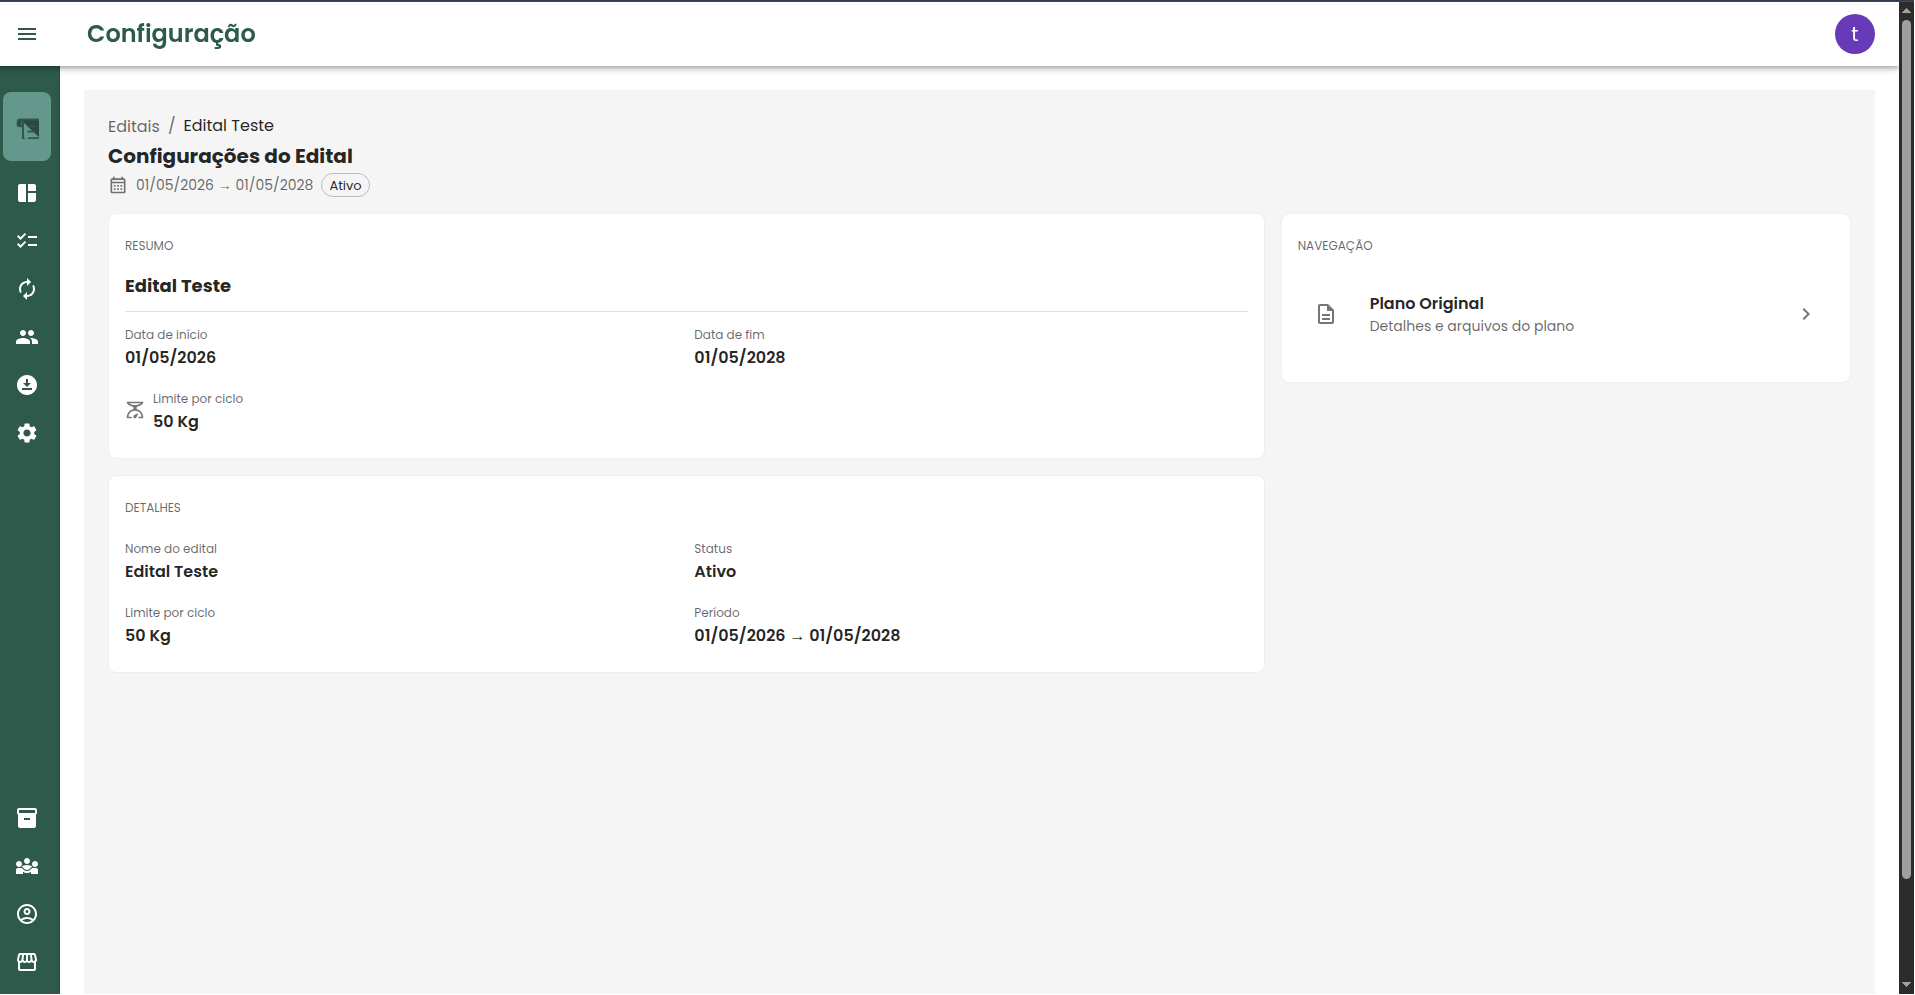
\includegraphics[width=1\textwidth]{Imagens/chap05/tela_configuracao_edital.png}
    \caption{Configuração}
    \label{fig:configuracao}
\end{figure}

Após a finalização do plano original, o dashboard passa a ser preenchido automaticamente com as informações necessárias para acompanhar o andamento do edital. A Figura~\ref{fig:dashboard} apresenta um exemplo da visualização dessa tela.

O dashboard é composto por indicadores que sintetizam o progresso. Entre essas informações, são apresentados os produtos cadastrados, a quantidade já entregue e a quantidade prevista no plano original. Ao interagir com um produto, por meio de um clique, o coordenador consegue visualizar a porcentagem de entrega correspondente a cada família, permitindo um acompanhamento mais detalhado da execução do edital.

Nessa mesma tela, também são apresentados dois gráficos relacionados ao andamento dos ciclos de entrega. O primeiro gráfico detalha quais produtos foram entregues em cada ciclo e suas respectivas quantidades. O segundo gráfico, localizado mais à direita, apresenta a quantidade total de alimentos entregue por ciclo, permitindo uma visão geral da evolução das entregas ao longo do edital.

\begin{figure}[H]
    \centering
    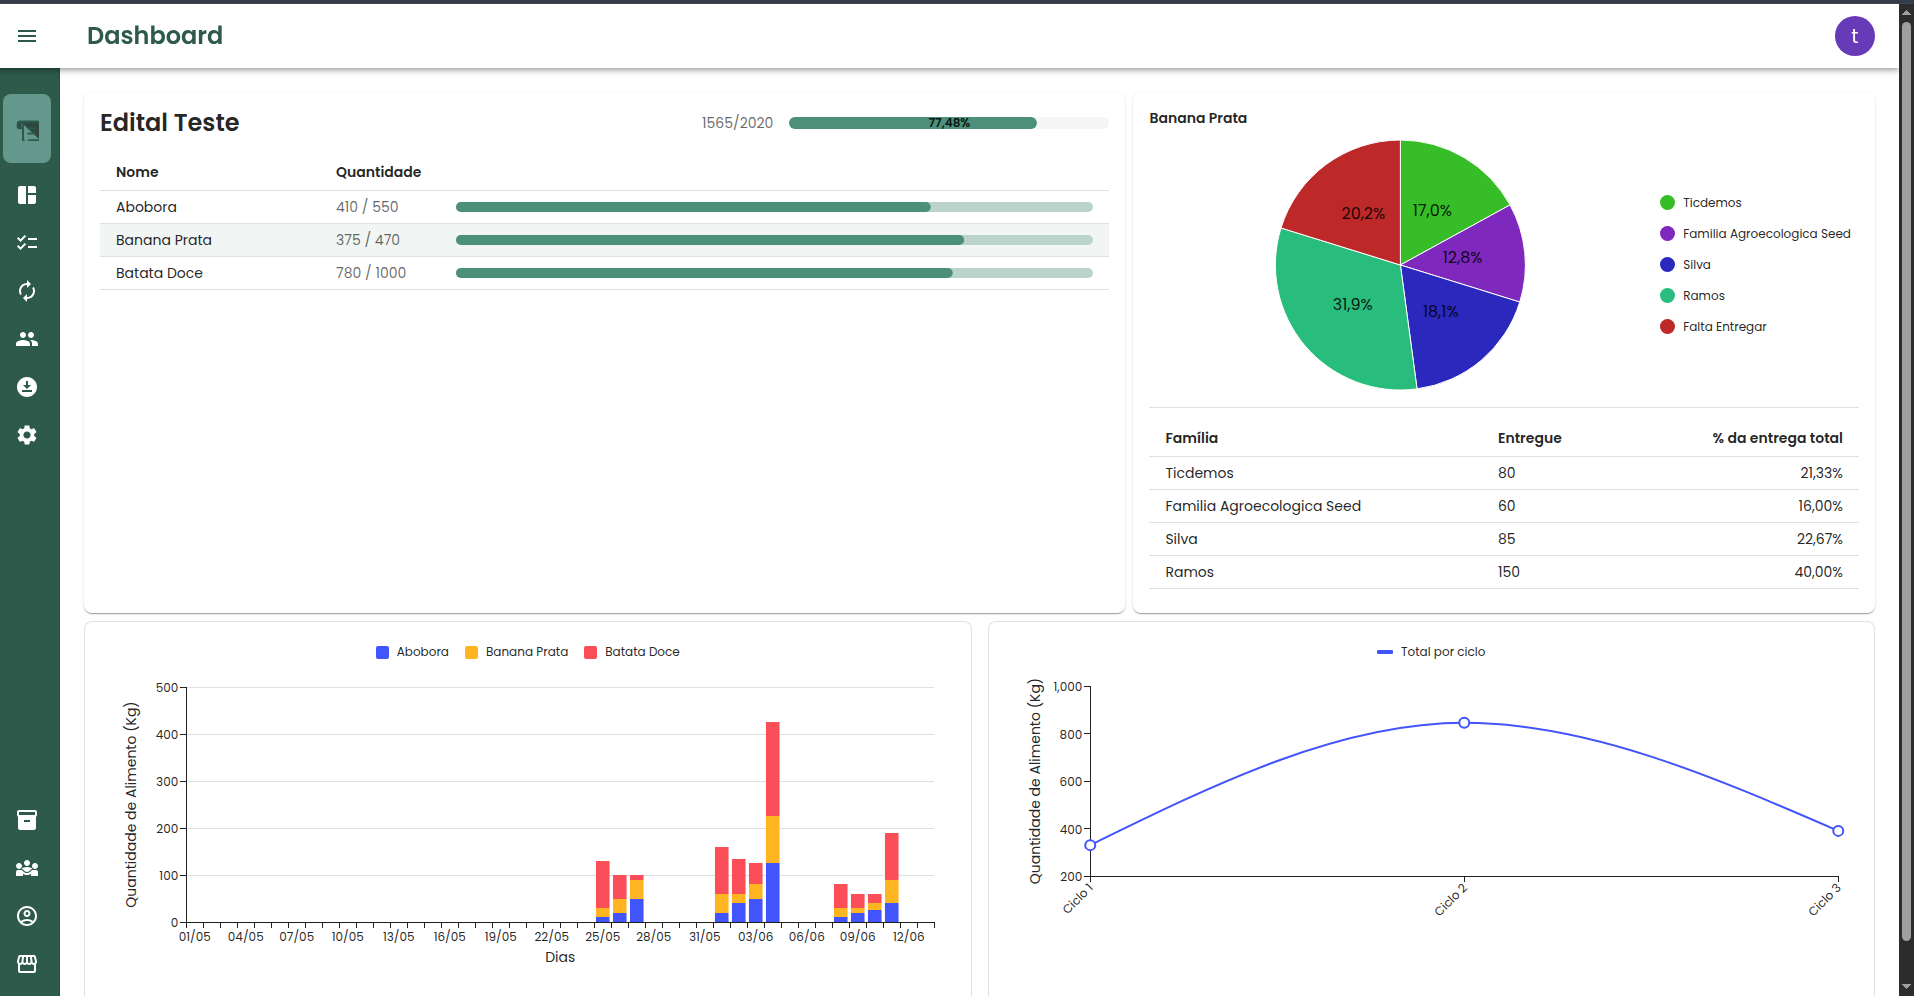
\includegraphics[width=1\textwidth]{Imagens/chap05/dashboard.png}
    \caption{Dashboard}
    \label{fig:dashboard}
\end{figure}

Com o objetivo de atender a informações comuns a diferentes editais, o sistema possui entidades globais, representadas nas figuras a seguir. Essas entidades evitam a repetição desnecessária de dados.

Na Figura~\ref{fig:produtos-globais}, são apresentados os produtos globais cadastrados no sistema. Cada edital pode possuir sua própria representação desses produtos, o que permite utilizar uma mesma informação base, mas com valores e quantidades específicas para cada edital. Dessa forma, um mesmo produto pode estar presente em diferentes editais, porém com preço, quantidade prevista e demais configurações próprias de cada chamada.

Além dos produtos, o sistema também possui como entidades globais os coletivos e os destinos, representados, respectivamente, pelas figuras~\ref{fig:coletivos-globais} e~\ref{fig:destinos-globais}. Esses cadastros permitem organizar informações utilizadas em diferentes partes do sistema, facilitando o gerenciamento e a vinculação dessas entidades aos editais.

Por fim, há também o cadastro de usuários, representado na Figura~\ref{fig:usuario-globais}. A partir dos usuários cadastrados, o sistema permite organizar os participantes e associá-los às famílias correspondentes, respeitando sua vinculação ao coletivo e à chamada pública correspondente.


\begin{figure}[H]
    \centering
    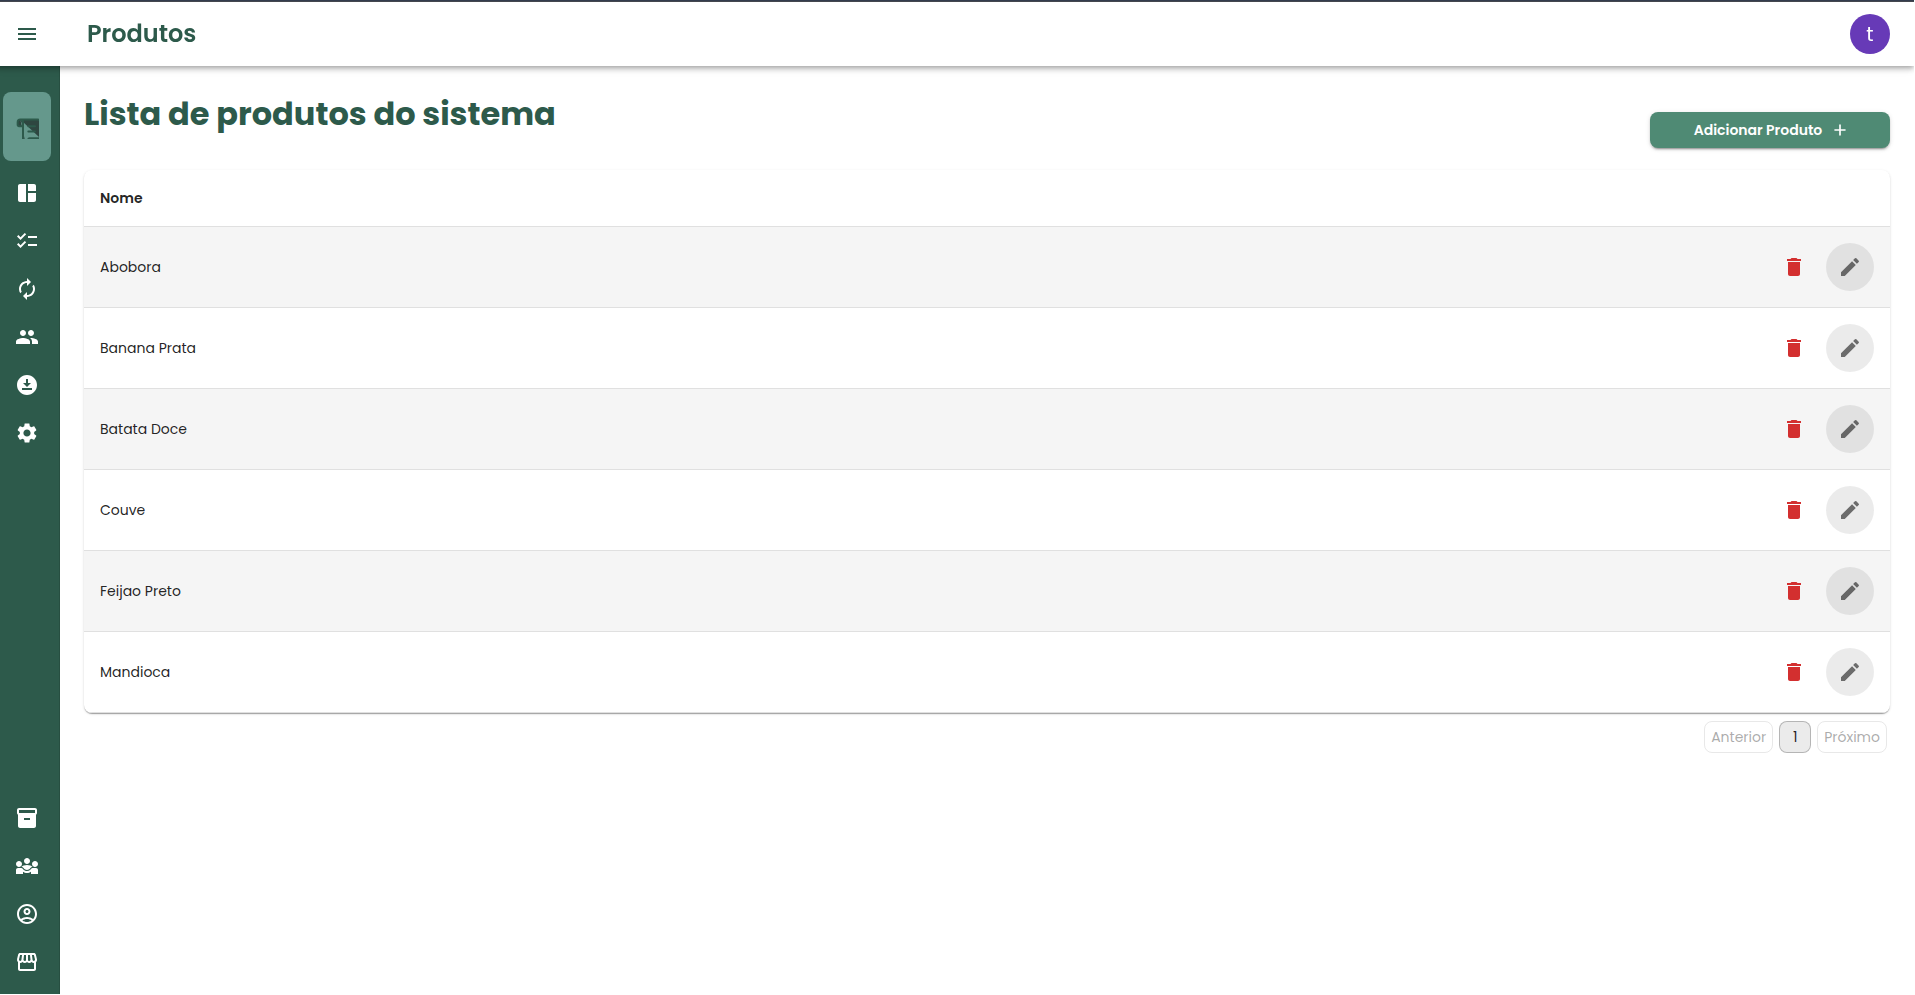
\includegraphics[width=1\textwidth]{Imagens/chap05/produtos_globais.png}
    \caption{Produtos}
    \label{fig:produtos-globais}
\end{figure}

\begin{figure}[H]
    \centering
    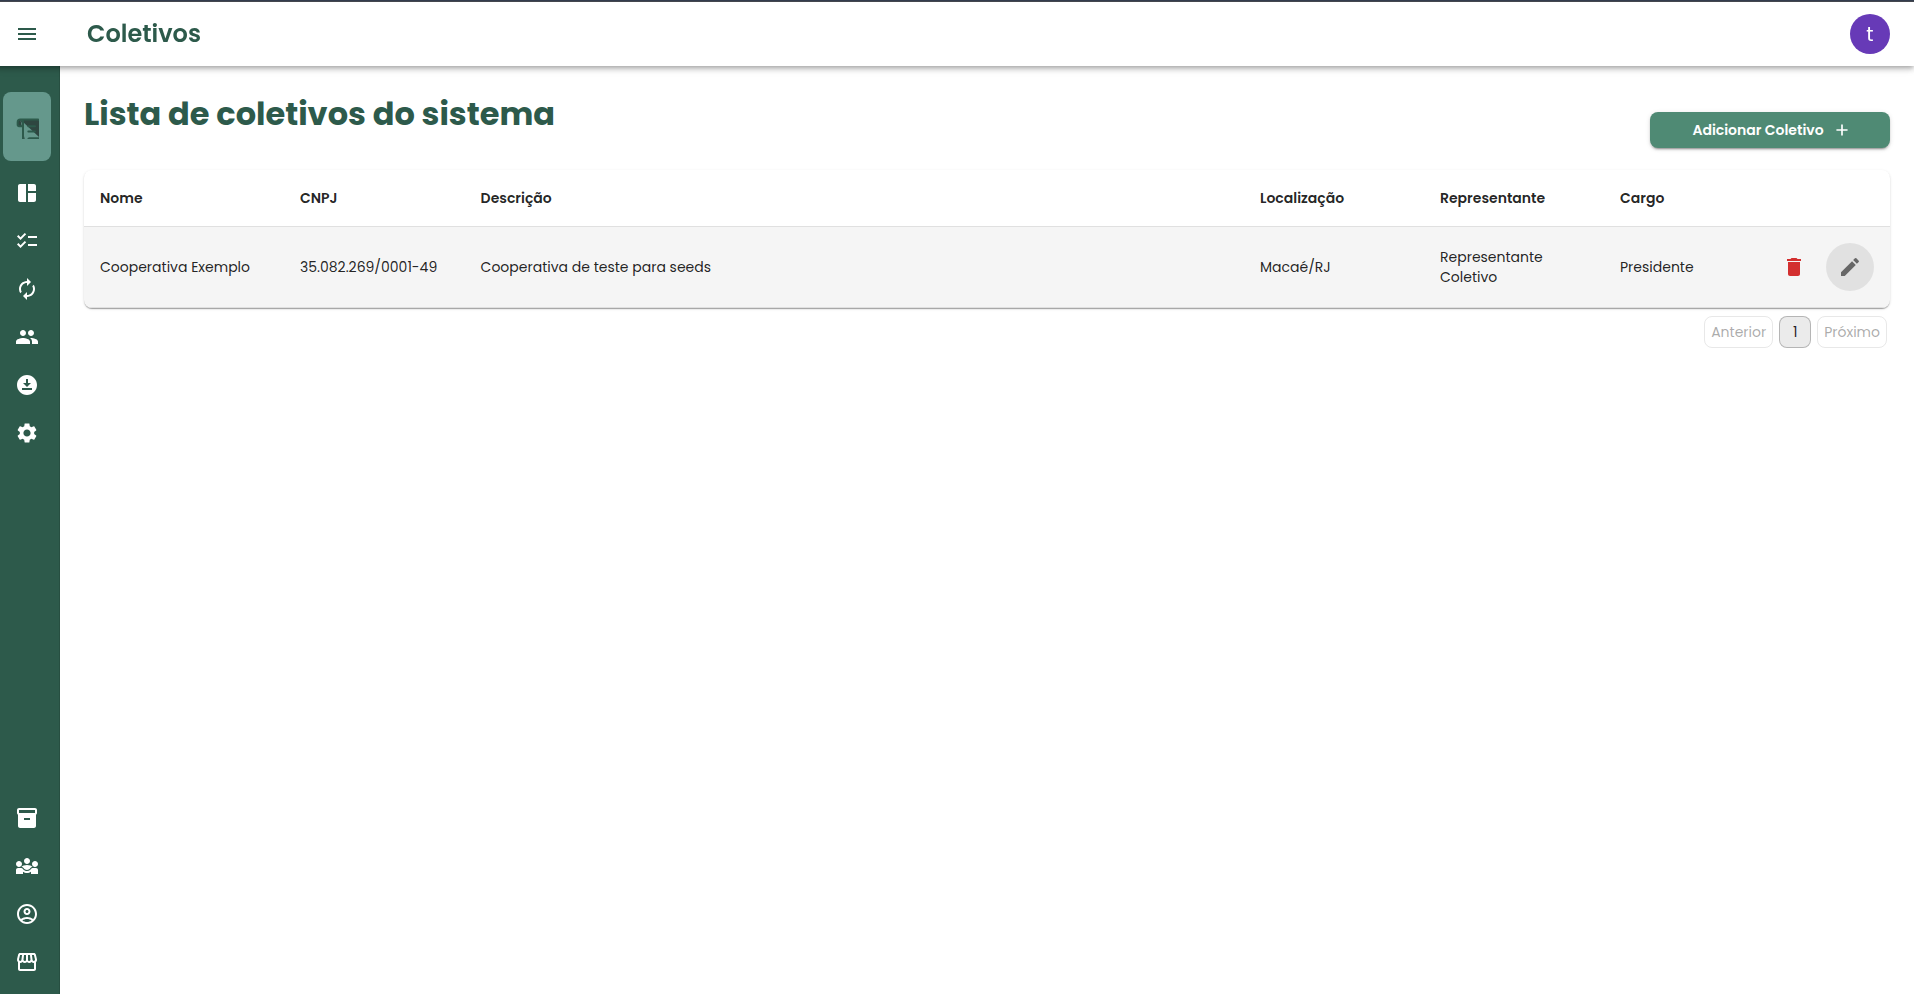
\includegraphics[width=1\textwidth]{Imagens/chap05/tela_coletivos.png}
    \caption{Coletivos}
    \label{fig:coletivos-globais}
\end{figure}

\begin{figure}[H]
    \centering
    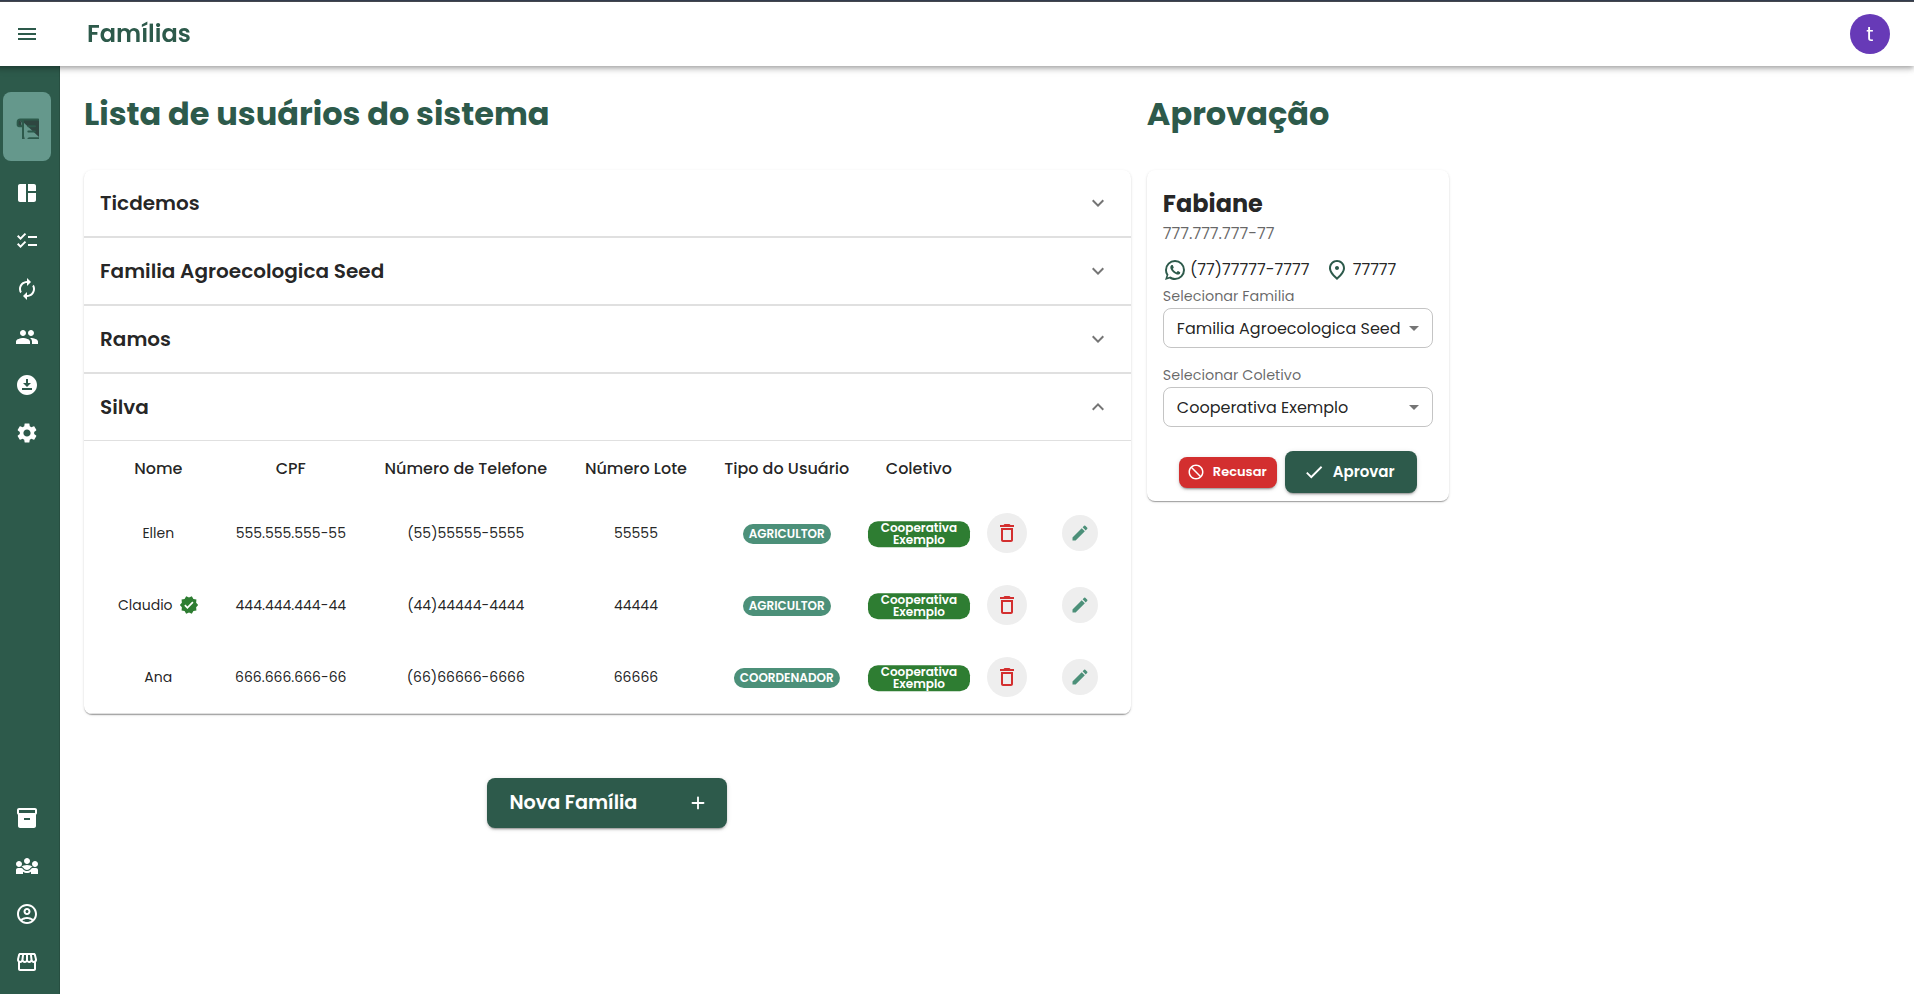
\includegraphics[width=1\textwidth]{Imagens/chap05/tela_usuarios_sistema.png}
    \caption{Usuários}
    \label{fig:usuario-globais}
\end{figure}

\begin{figure}[H]
    \centering
    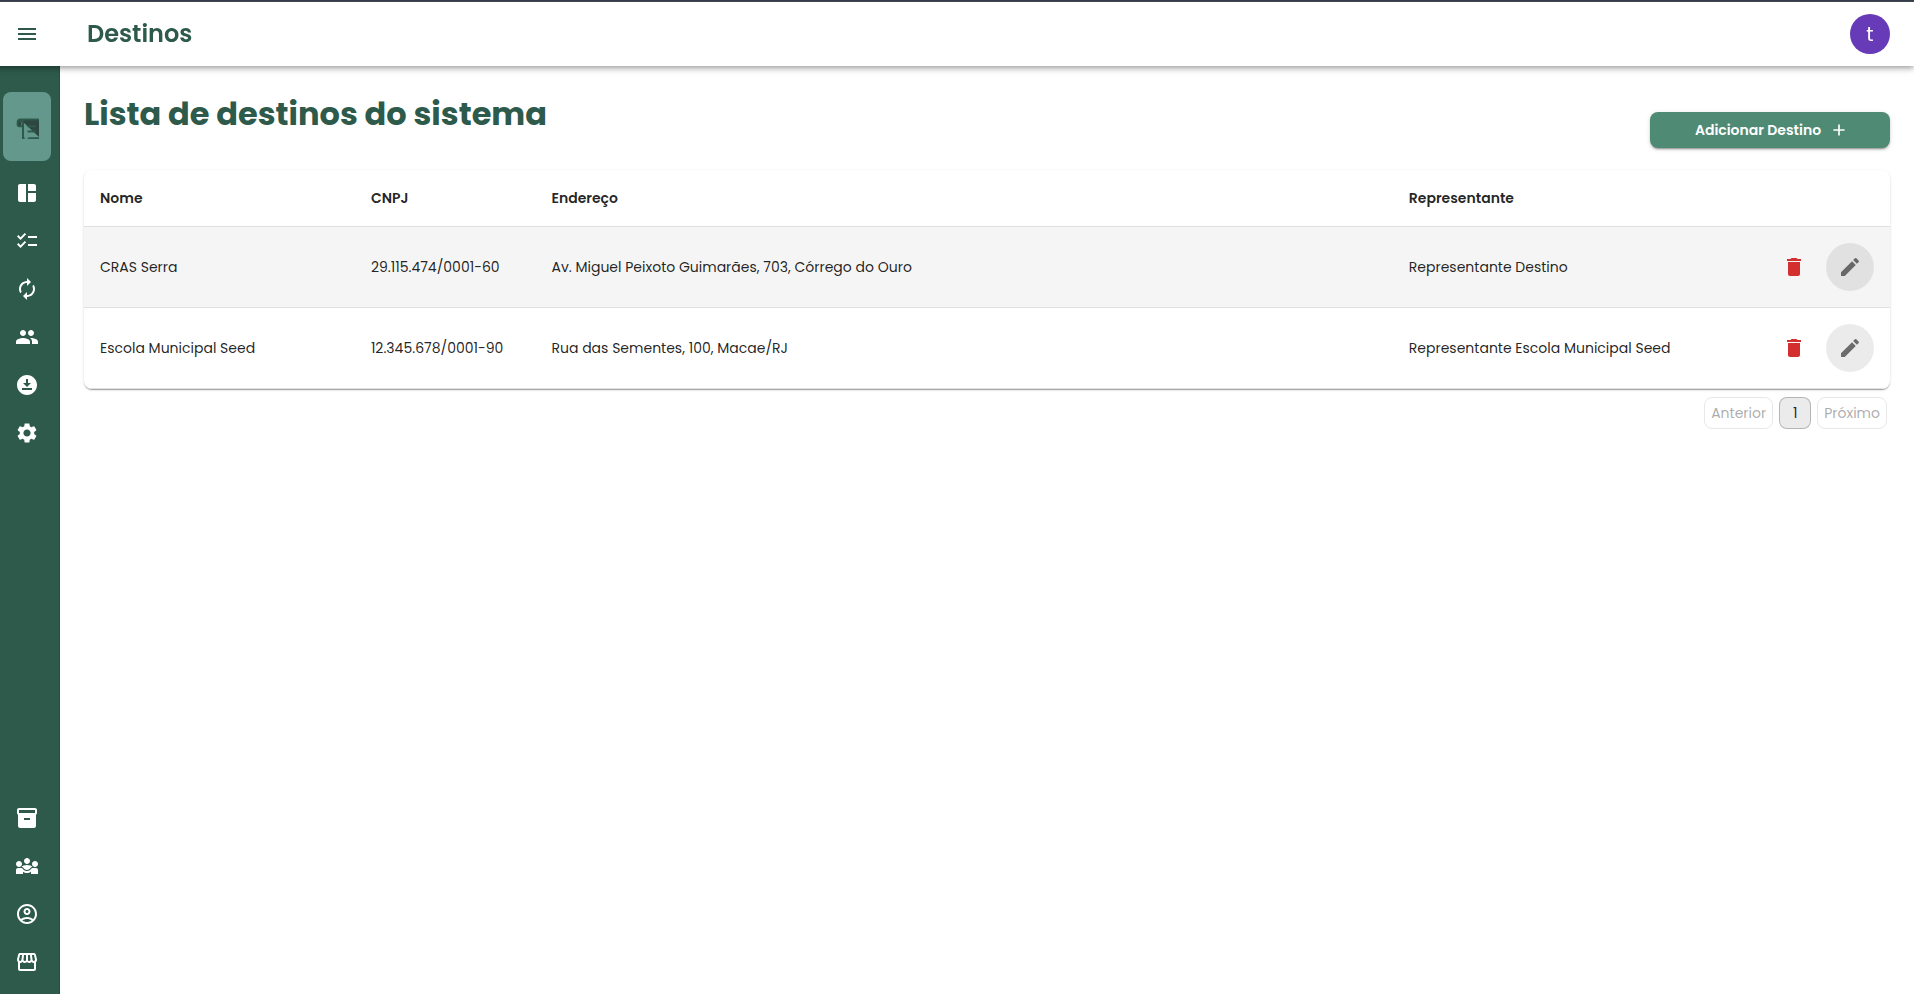
\includegraphics[width=1\textwidth]{Imagens/chap05/tela_destino_sistema.png}
    \caption{Destinos}
    \label{fig:destinos-globais}
\end{figure}

\section{Integração e Deploy}

Durante o desenvolvimento do sistema, foi utilizado o Git como ferramenta de controle de versão, permitindo o acompanhamento das alterações realizadas no código-fonte e facilitando o trabalho colaborativo entre os desenvolvedores. Para o armazenamento remoto dos repositórios, foi utilizado o GitLab, que também oferece recursos de integração contínua e entrega contínua.

Com o objetivo de apoiar a integração contínua de novas funcionalidades e padronizar o processo de construção da aplicação, foi configurado, em cada projeto, um arquivo chamado \texttt{.gitlab-ci.yml}. Esse arquivo é responsável por definir as etapas executadas automaticamente pelo GitLab CI/CD, como a verificação do código, acionamento de testes automatizados, a execução do build e a geração de uma nova imagem Docker. No backend, esse processo utiliza o Maven para executar as etapas de teste e construção da aplicação. No frontend, o processo utiliza o Vite para gerar a versão de produção da interface. Neste primeiro momento a aplicação possui somente testes automatizados para pontos essenciais e comportamentos críticos do sistema. Após a criação da imagem, ela é publicada no Docker Hub, possibilitando que a versão mais recente da aplicação esteja disponível para implantação no ambiente de homologação.

O ambiente de homologação da aplicação encontra-se em uma VPS hospedada na Hostinger. Nesse ambiente, o deploy ainda é realizado de forma manual. Para isso, existe um script no servidor responsável por remover as imagens locais dos containers, baixar as versões mais recentes publicadas no Docker Hub e executar novamente o Docker Compose, fazendo com que os serviços da aplicação sejam atualizados e disponibilizados online.



\clearpage{}
    \clearpage{}\chapter{Resultados}
\label{chap6}

Atualmente, o sistema encontra-se em fase de homologação. Essa etapa tem como objetivo validar, junto aos usuários envolvidos no processo de gestão do PAA e ao Assentamento PDS Osvaldo de Oliveira, se as funcionalidades implementadas atendem às necessidades identificadas durante o levantamento de requisitos e se o fluxo do sistema corresponde à realidade operacional do programa.

A versão em homologação contempla as principais funcionalidades necessárias para a criação e o acompanhamento de um edital, permitindo organizar informações que antes eram controladas de forma manual, principalmente por meio de planilhas. Entre essas funcionalidades, destacam-se o cadastro de usuários, a aprovação de acesso ao sistema, o cadastro de famílias, a criação de editais e a definição dos perfis de acesso dos participantes.

Com isso, é possível observar que o sistema propõe uma nova forma de olhar para a gestão do PAA. Ao centralizar as informações em uma plataforma web, o acompanhamento dos editais tende a se tornar mais objetivo, claro e transparente. Além disso, a ferramenta reduz a dependência de controles manuais e facilita a consulta das informações pelos diferentes usuários envolvidos no processo.

Dessa forma, mesmo ainda estando em homologação, o sistema já demonstra potencial para contribuir com a organização da gestão do PAA no assentamento. A validação com os usuários será fundamental para identificar ajustes necessários, melhorar a experiência de uso e garantir que a ferramenta esteja adequada às demandas reais da comunidade antes de sua implantação definitiva.


\clearpage{}
    \clearpage{}\chapter{Conclusão}
\label{chap7}

\section{Conclusão}

O desenvolvimento deste trabalho permitiu a construção de um sistema web voltado ao apoio da gestão do Programa de Aquisição de Alimentos na modalidade Doação Simultânea, tendo como referência o contexto do Assentamento PDS Osvaldo de Oliveira. A proposta partiu de uma necessidade concreta: reduzir a dependência de controles manuais, centralizar informações da chamada pública e facilitar o acompanhamento das entregas realizadas pelas famílias agricultoras aos destinos vinculados ao edital. Ao longo do processo, o sistema deixou de ser apenas uma ideia inicial e passou a constituir uma aplicação em fase de homologação, com funcionalidades implementadas e com possibilidade de validação junto aos usuários envolvidos.

Entre os resultados alcançados, destacam-se a implementação de fluxos essenciais para o funcionamento da plataforma, funcionalidades que representam uma base importante para a gestão do PAA, pois permitem organizar informações que antes eram acompanhadas principalmente por planilhas e registros manuais. Do ponto de vista técnico, o trabalho atingiu um resultado relevante ao estruturar a aplicação em módulos separados, com contextos bem definidos. A escolha por uma arquitetura modular favoreceu a independência entre a interface e as regras de negócio, permitindo que novas funcionalidades fossem incorporadas de forma progressiva.

Além da implementação, o projeto evidenciou a importância de aproximar o desenvolvimento de software do contexto social em que a ferramenta será utilizada. O levantamento de requisitos, as reuniões com os gestores do PAA e os ajustes realizados a partir de novas demandas evidenciam que a construção de uma solução não depende apenas da escolha de tecnologias, mas também da compreensão do processo real de trabalho, agregando valor o que foi desenvolvido.

Os trabalhos futuros devem partir da análise do que já foi implementado e do estágio atual do sistema. Para as novas implementações, a metodologia participativa deverá continuar presente, para que o software tenha maior aderência aos usuários e faça diferença no dia a dia dos coordenadores, administradores e agricultores. A análise da arquitetura planejada e implementada indica que ela atende a uma demanda simples. No entanto, em um contexto mais amplo, considerando o Brasil, o sistema deverá implementar métricas de desempenho, reforçar a segurança dos dados, dividir funcionalidades em serviços e contar com uma estrutura capaz de suportar milhares de requisições, caso seja necessário.

Por fim, conclui-se que este trabalho contribui tanto para a organização técnica de uma aplicação web quanto para a construção de uma ferramenta voltada a uma demanda social específica. O sistema desenvolvido oferece uma base para tornar a gestão das chamadas públicas mais transparente, menos dependente de processos manuais e mais próxima das necessidades dos usuários. Ao mesmo tempo, sua continuidade exigirá novas etapas de amadurecimento, especialmente para que a solução possa deixar de ser apenas um sistema em homologação e se tornar uma ferramenta estável.


\clearpage{}
  \backmatter
  \nocite{*}
  \bibliographystyle{IEEEtranM}
  \bibliography{thesis}
  \appendix
  \chapter{Diagramas UML de casos de uso}
\label{apendice-casos-uso}

Este apêndice apresenta os diagramas UML correspondentes aos principais casos de uso do sistema Biribá. As funcionalidades foram agrupadas por área para evidenciar as associações dos atores agricultor, coordenador e administrador com o sistema, sem omitir nenhum dos casos de uso identificados no levantamento de requisitos.

\tikzset{
    uml system/.style={draw, rounded corners=2pt, fill=gray!4},
    uml use case/.style={
        draw,
        ellipse,
        fill=white,
        align=center,
        font=\small,
        minimum width=4.4cm,
        minimum height=0.95cm
    },
    uml association/.style={draw, semithick},
    pics/uml actor/.style args={#1}{
        code={
            \draw (0,0.65) circle (0.17);
            \draw (0,0.48) -- (0,-0.12);
            \draw (-0.32,0.27) -- (0.32,0.27);
            \draw (0,-0.12) -- (-0.27,-0.58);
            \draw (0,-0.12) -- (0.27,-0.58);
            \node[font=\small, align=center, anchor=north] at (0,-0.72) {#1};
            \coordinate (-center) at (0,0.15);
        }
    }
}

\section{Acesso ao sistema}

A Figura~\ref{fig:uc-acesso} representa a solicitação de cadastro pelo agricultor e a aprovação ou rejeição desse acesso pelo coordenador ou administrador.

\begin{figure}[H]
    \centering
    \begin{tikzpicture}
        \node[uml system, minimum width=8.4cm, minimum height=4.2cm] (sistema) at (7.5,0) {};
        \node[anchor=north west, font=\small\bfseries] at ([xshift=0.2cm,yshift=-0.15cm]sistema.north west) {Sistema Biribá};

        \node[uml use case] (solicitar) at (7.5,1) {Solicitar cadastro};
        \node[uml use case] (aprovar) at (7.5,-1) {Aprovar usuário};

        \pic (agricultor) at (1.4,1) {uml actor={Agricultor}};
        \pic (coordenador) at (1.4,-1) {uml actor={Coordenador}};
        \pic (administrador) at (13.6,-1) {uml actor={Administrador}};

        \draw[uml association] (agricultor-center) -- (solicitar.west);
        \draw[uml association] (coordenador-center) -- (aprovar.west);
        \draw[uml association] (administrador-center) -- (aprovar.east);
    \end{tikzpicture}
    \caption{Diagrama UML dos casos de uso de acesso ao sistema}
    \label{fig:uc-acesso}
\end{figure}

\section{Configuração do edital}

A Figura~\ref{fig:uc-configuracao} apresenta os casos de uso associados à preparação da chamada pública. O coordenador e o administrador podem gerenciar famílias, criar editais e criar ciclos de entrega, enquanto o gerenciamento global de produtos e destinos é atribuído ao administrador.

\begin{figure}[H]
    \centering
    \begin{tikzpicture}
        \node[uml system, minimum width=8.6cm, minimum height=7.2cm] (sistema) at (7.5,0) {};
        \node[anchor=north west, font=\small\bfseries] at ([xshift=0.2cm,yshift=-0.15cm]sistema.north west) {Sistema Biribá};

        \node[uml use case] (familias) at (7.5,2.35) {Gerenciar famílias};
        \node[uml use case] (edital) at (7.5,1.18) {Criar edital};
        \node[uml use case] (produtos) at (7.5,0) {Gerenciar produtos};
        \node[uml use case] (destinos) at (7.5,-1.18) {Gerenciar destinos};
        \node[uml use case] (ciclos) at (7.5,-2.35) {Criar ciclos de entrega};

        \pic (coordenador) at (1.3,0.7) {uml actor={Coordenador}};
        \pic (administrador) at (13.7,-0.1) {uml actor={Administrador}};

        \draw[uml association] (coordenador-center) -- (familias.west);
        \draw[uml association] (coordenador-center) -- (edital.west);
        \draw[uml association] (coordenador-center) -- (ciclos.west);

        \draw[uml association] (administrador-center) -- (familias.east);
        \draw[uml association] (administrador-center) -- (edital.east);
        \draw[uml association] (administrador-center) -- (produtos.east);
        \draw[uml association] (administrador-center) -- (destinos.east);
        \draw[uml association] (administrador-center) -- (ciclos.east);
    \end{tikzpicture}
    \caption{Diagrama UML dos casos de uso de configuração do edital}
    \label{fig:uc-configuracao}
\end{figure}

\section{Execução e acompanhamento}

A Figura~\ref{fig:uc-execucao} representa as funcionalidades utilizadas durante a execução do edital. O coordenador e o administrador registram entregas, acompanham os indicadores e geram relatórios, enquanto o agricultor consulta os dados referentes à sua participação.

\begin{figure}[H]
    \centering
    \begin{tikzpicture}
        \node[uml system, minimum width=8.6cm, minimum height=6.3cm] (sistema) at (7.5,0) {};
        \node[anchor=north west, font=\small\bfseries] at ([xshift=0.2cm,yshift=-0.15cm]sistema.north west) {Sistema Biribá};

        \node[uml use case] (entrega) at (7.5,1.8) {Registrar entrega};
        \node[uml use case] (dashboard) at (7.5,0.6) {Acompanhar dashboard};
        \node[uml use case] (relatorios) at (7.5,-0.6) {Gerar relatórios};
        \node[uml use case] (consulta) at (7.5,-1.8) {Consultar informações\\da participação};

        \pic (coordenador) at (1.3,0.6) {uml actor={Coordenador}};
        \pic (administrador) at (13.7,0.6) {uml actor={Administrador}};
        \pic (agricultor) at (1.3,-1.8) {uml actor={Agricultor}};

        \draw[uml association] (coordenador-center) -- (entrega.west);
        \draw[uml association] (coordenador-center) -- (dashboard.west);
        \draw[uml association] (coordenador-center) -- (relatorios.west);

        \draw[uml association] (administrador-center) -- (entrega.east);
        \draw[uml association] (administrador-center) -- (dashboard.east);
        \draw[uml association] (administrador-center) -- (relatorios.east);

        \draw[uml association] (agricultor-center) -- (consulta.west);
    \end{tikzpicture}
    \caption{Diagrama UML dos casos de uso de execução e acompanhamento}
    \label{fig:uc-execucao}
\end{figure}

\section{Administração da plataforma}

A Figura~\ref{fig:uc-administracao} apresenta o caso de uso de manutenção da plataforma, reservado ao administrador e relacionado aos ajustes, às correções e à evolução do sistema.

\begin{figure}[H]
    \centering
    \begin{tikzpicture}
        \node[uml system, minimum width=8.4cm, minimum height=3cm] (sistema) at (7.5,0) {};
        \node[anchor=north west, font=\small\bfseries] at ([xshift=0.2cm,yshift=-0.15cm]sistema.north west) {Sistema Biribá};

        \node[uml use case] (manter) at (7.5,0) {Manter o sistema};
        \pic (administrador) at (1.4,0) {uml actor={Administrador}};

        \draw[uml association] (administrador-center) -- (manter.west);
    \end{tikzpicture}
    \caption{Diagrama UML do caso de uso de administração da plataforma}
    \label{fig:uc-administracao}
\end{figure}

\end{document}
